%%%%%%%%%%%%%%%%%%%%%%%%%%%%%%%%%%%%
%                                  %
% Titre  : p_l.tex                 %
% Sujet  : Manuel de l'utilisateur %
%          du projet 'PT-Scotch'   %
%          Bibliotheque            %
% Auteur : Francois Pellegrini     %
%                                  %
%%%%%%%%%%%%%%%%%%%%%%%%%%%%%%%%%%%%

\section{Library}
\label{sec-lib}

All of the features provided by the programs of the
\ptscotch\ distribution may be directly accessed by calling
the appropriate functions of the \libscotch\ library, archived
in files {\tt libptscotch.a} and {\tt libptscotcherr.a}.
All of the existing parallel routines belong to four distinct classes:
\begin{itemize}
\item
distributed source graph handling routines, which serve to declare,
build, load, save, and check the consistency of distributed source
graphs;
%, along with their geometry data;
\item
strategy handling routines, which allow the user to declare and build
parallel mapping and ordering strategies;
\item
parallel graph partitioning and static mapping routines, which allow
the user to declare, compute, and save distributed static mappings of
distributed source graphs;
\item
parallel ordering routines, which allow the user to declare, compute,
and save distributed orderings of distributed source graphs.
\end{itemize}
Error handling is performed using the existing sequential routines of
the \scotch\ distribution, which are described in the
{\it\scotch\ User's Guide}~\scotchcitesuser. Their use is recalled in
Section~\ref{sec-lib-error}.

A \parmetis\ compatibility library, called {\tt lib\lbo ptscotch\lbo
parmetis.a}, is also available. It allows users who were previously
using \parmetis\ in their software to take advantage of the efficieny
of \ptscotch\ without having to modify their code. The services
provided by this library are described in
Section~\ref{sec-lib-parmetis}.

\subsection{Running at proper thread level}
\label{sec-lib-thread}

Since \ptscotch\ is based on the MPI API, all processes must call some
flavor of \texttt{MPI\_\lbt Init} before using any routine of the
library that performs communication. The thread support level of MPI
has to be set in accordance to the level required by the library.

If \ptscotch\ has been compiled without the \texttt{-DSCOTCH\_\lbt
PTHREAD} flag, a call to the simple \texttt{MPI\_\lbt Init} routine
will suffice, because no concurrent MPI calls will be performed by
library routines. Else, the extended \texttt{MPI\_\lbt Init\_\lbt
thread} initialization routine has to be used, to request the
\texttt{MPI\_\lbt THREAD\_\lbt MULTIPLE} level, and the provided
thread support level value returned by the routine must be checked
carefully. If your MPI implementation does not provide the
\texttt{MPI\_\lbt THREAD\_\lbt MULTIPLE} level, you will have to
recompile \ptscotch\ without the \texttt{-DSCOTCH\_\lbt PTHREAD}
flag. Else, library calls may cause random bugs in the communication
subsystem, resulting in program crashes.

\subsection{Calling the routines of {\sc libScotch}}

\subsubsection{Calling from C}

All of the C routines of the \libscotch\ library are prefixed with
``{\tt SCOTCH\_}''. The remainder of the function names is made of the
name of the type of object to which the functions apply (e\@.g\@.
``{\tt dgraph}'', ``{\tt dorder}'', etc.),
followed by the type of action performed on this object: ``{\tt
Init}'' for the initialization of the object, ``{\tt Exit}'' for the
freeing of its internal structures, ``{\tt Load}'' for loading the
object from one or several streams, and so on.

Typically, functions that return an error code return zero if the
function succeeds, and a non-zero value in case of error.

For instance, the {\tt SCOTCH\_\lbt dgraph\lbt Init} and {\tt
SCOTCH\_\lbt dgraph\lbt Load} routines, described in
section~\ref{sec-lib-dgraph}, can be called from C by using the
following code.
{\tt
\begin{verbatim}
#include <stdio.h>
#include <mpi.h>
#include "ptscotch.h"
  ...
  SCOTCH_Dgraph     grafdat;
  FILE *            fileptr;

  if (SCOTCH_dgraphInit (&grafdat) != 0) {
    ... /* Error handling */
  }
  if ((fileptr = fopen ("brol.grf", "r")) == NULL) {
  ... /* Error handling */
  }
  if (SCOTCH_dgraphLoad (&grafdat, fileptr, -1, 0) != 0) {
    ... /* Error handling */
  }
  ...
\end{verbatim}
}

Since ``{\tt ptscotch.h}'' uses several system and communication
objects which are declared in ``{\tt stdio.h}'' and ``{\tt mpi.h}'',
respectively, these latter files must be included beforehand
in your application code.

Although the ``{\tt scotch.h}'' and ``{\tt ptscotch.h}'' files may
look very similar on your system, never mistake them, and always use
the ``{\tt ptscotch.h}'' file as the right include file for compiling
a program which uses the parallel routines of the \libscotch\ library,
whether it also calls sequential routines or not.

\subsubsection{Calling from Fortran}

The routines of the \libscotch\ library can also be called from
Fortran. For any C function named {\tt SCOTCH\_\lbt {\it type\lbt
Action}()} which is documented in this manual, there exists a {\tt
SCOTCHF\lbt {\it TYPE\lbt ACTION\/}()} Fortran counterpart, in which
the separating underscore character is replaced by an ``{\tt
F}''. In most cases, the Fortran routines have exactly the same
parameters as the C functions, save for an added trailing {\tt
INTEGER} argument to store the return value yielded by the function
when the return type of the C function is not {\tt void}.
\\

Since all the data structures used in \libscotch\ are
opaque, equivalent declarations for these structures must
be provided in Fortran. These structures must therefore
be defined as arrays of {\tt DOUBLEPRECISION}s, of sizes
given in file {\tt ptscotchf.h}, which must be included whenever
necessary.

For routines that read or write data using a {\tt FILE~*} stream
in C, the Fortran counterpart uses an {\tt INTEGER} parameter which
is the numer of the Unix file descriptor corresponding to the logical
unit from which to read or write. In most Unix implementations of
Fortran, standard descriptors 0 for standard input (logical unit 5),
1 for standard output (logical unit 6) and 2 for standard error are
opened by default. However, for files that are opened using
{\tt OPEN} statements, an additional function must be used to obtain
the number of the Unix file descriptor from the number of the logical
unit. This function is called \texttt{PXFFILENO} in the normalized
POSIX Fortran API, and files which use it should include the
\texttt{USE IFPOSIX} directive whenever necessary. An alternate, non
normalized, function also exists in most Unix implementations of
Fortran, and is called {\tt FNUM}.

For instance, the {\tt SCOTCH\_\lbt dgraph\lbt Init} and
{\tt SCOTCH\_\lbt dgraph\lbt Load} routines, described in
sections~\ref{sec-lib-dgraphinit} and~\ref{sec-lib-dgraphload},
respectively, can be called from Fortran by using the following code.
{\tt
\begin{verbatim}
        INCLUDE "ptscotchf.h"
        DOUBLEPRECISION GRAFDAT(SCOTCH_DGRAPHDIM)
        INTEGER RETVAL
        ...
        CALL SCOTCHFDGRAPHINIT (GRAFDAT (1), RETVAL)
        IF (RETVAL .NE. 0) THEN
        ...
        OPEN (10, FILE='brol.grf')
        CALL SCOTCHFDGRAPHLOAD (GRAFDAT (1), PXFFILENO (10), 1, 0, RETVAL)
        CLOSE (10)
        IF (RETVAL .NE. 0) THEN
        ...
\end{verbatim}
}

Although the ``{\tt scotchf.h}'' and ``{\tt ptscotchf.h}'' files may
look very similar on your system, never mistake them, and always use
the ``{\tt ptscotchf.h}'' file as the include file for compiling a
Fortran program that uses the parallel routines of the
\libscotch\ library, whether it also calls sequential routines or not.

All of the Fortran routines of the \libscotch\ library are stubs which
call their C counterpart. While this poses no problem for the usual
integer and double precision data types, some conflicts may occur at
compile or run time if your MPI implementation does not represent the
{\tt MPI\_Comm} type in the same way in C and in Fortran. Please check
on your platform to see in the {\tt mpi.h} include file if the {\tt
MPI\_Comm} data type is represented as an {\tt int}. If it is the
case, there should be no problem in using the Fortran routines of
the \ptscotch\ library.

\subsubsection{Compiling and linking}

The compilation of C or Fortran routines which use parallel
routines of the \libscotch\ library requires that either {\tt
ptscotch.h} or {\tt ptscotchf.h} be included, respectively. Since some
of the parallel routines of the \libscotch\ library must be passed MPI
communicators, it is necessary to include MPI files {\tt mpi.h} or
{\tt mpif.h}, respectively, before the relevant \ptscotch\ include
files, such that prototypes of the parallel \libscotch\ routines are
properly defined.

The parallel routines of the \libscotch\ library, along with
taylored versions of the sequential routines, are grouped in a
library file called {\tt libptscotch.a}. Default error routines that
print an error message and exit are provided in the classical
\scotch\ library file {\tt libptscotcherr.a}.

Therefore, the linking of applications that make use of the
\libscotch\ library with standard error handling is carried out by
using the following options: ``{\tt -lptscotch -lptscotcherr -lmpi -lm}''.
The ``{\tt -lmpi}'' option is most often not necessary, as the MPI
library is automatically considered when compiling with commands such
as {\tt mpicc}.

If you want to handle errors by yourself, you should not link with
library file {\tt libptscotcherr.a}, but rather provide a
{\tt SCOTCH\_\lbt error\lbt Print()} routine. Please refer to
Section~\ref{sec-lib-error} for more information on error handling.
Section~\ref{sec-lib-error} for more information on error handling.

Programs that use both sequential and parallel routines of
\scotch\ need only be linked against the parallel version of the
library, as it also contains an adapted version of the sequential
routines. The reason why the sequential routines are duplicated in the
parallel \ptscotch\ library is because they are slightly modified so
as to keep track of the parallel environment. This allows one to
create ``multi-sequential'' routines that can exchange data with other
processes, for instance. Because the \libscotch\ data structures
contain extra parameters, never mix the \texttt{scotch.h} sequential
include file and the \texttt{libptscotch.a} parallel library, as the
latter expects \scotch\ data structures to be larger than the ones
defined in the sequential include file. Consequently, when using only
sequential routines in a sequential program, include the
\texttt{scotch.h} file only and link the program against the sequential
\texttt{libscotch.a} library only. When using only parallel routines,
or when using a mix of sequential and parallel routines, include the
\texttt{ptscotch.h} file only and link the program against the parallel
\texttt{libptscotch.a} library only. When using only sequential
routines in a parallel program, both options can be used.

\subsubsection{Machine word size issues}
\label{sec-lib-inttypesize}

Graph indices are represented in \scotch\ as integer values of type
{\tt SCOTCH\_\lbt Num}. By default, this type equates to the {\tt int}
C type, that is, an integer type of size equal to the one of 
the machine word. However, it can represent any other integer
type. Indeed, the size of the {\tt SCOTCH\_\lbt Num} integer type can
be coerced to 32 or 64 bits by using the ``{\tt -DINTSIZE32}'' or
``{\tt -DINTSIZE64}'' compilation flags, respectively, or else by
using the ``{\tt -DINT=}'' definition (see
Section~\ref{sec-install-inttypesize} for more information on the
setting of these compilation flags).

This may, however, pose a problem with MPI, the interface of which is
based on the regular {\tt int} type. \ptscotch\ has been coded so
as to avoid typecast bugs, but overflow errors may result from the
conversion of values of a larger integer type into {\tt int}s when
handling communication buffer indices.

Consequently, the C interface of \scotch\ uses two types of integers.
Graph-related quantities are passed as {\tt SCOTCH\_\lbt Num}s,
while system-related values such as file handles, as well as
return values of \libscotch\ routines, are always passed as
{\tt int}s.

Because of the variability of library integer type sizes, one must be
careful when using the Fortran interface of \scotch, as it does not
provide any prototyping information, and consequently cannot produce
any warning at link time. In the manual pages of the
\libscotch\ routines, Fortran prototypes are written using three types
of {\tt INTEGER}s. As for the C interface, the regular {\tt INTEGER}
type is used for system-based values, such as file handles and MPI
communicators, as well as for return values of the
\libscotch\ routines, while the {\tt INTEGER*}{\it num} type
should be used for all graph-related values, in accordance to the size
of the {\tt SCOTCH\_\lbt Num} type, as set by the
``{\tt -DINTSIZE}{\it x}'' compilation flags. Also, the
{\tt INTEGER*}{\it idx} type represents an integer type of a size
equivalent to the one of a {\tt SCOTCH\_\lbt Idx}, as set by the
``{\tt -DIDXSIZE}{\it x}'' compilation flags. Values of this type are
used in the Fortran interface to represent arbitrary array indices
which can span across the whole address space, and consequently
deserve special treatment.

In practice, when \scotch\ is compiled on a 32-bit architecture so as
to use 64-bit {\tt SCOTCH\_\lbt Num}s, graph indices should be
declared as {\tt INTEGER*8}, while error return values
should still be declared as plain {\tt INTEGER} (that is,
{\tt INTEGER*4}) values. On a 32\_64-bit architecture, irrespective of
whether {\tt SCOTCH\_\lbt Num}s are defined as {\tt INTEGER*4}
or {\tt INTEGER*8} quantities, the {\tt SCOTCH\_\lbt Idx} type
should always be defined as a 64-bit quantity, that is, an
{\tt INTEGER*8}, because it stores differences between memory
addresses, which are represented by 64-bit values.
The above is no longer a problem if \scotch\ is compiled such that
{\tt int}s equate 64-bit integers. In this case, there is no need to
use any type coercing definition.
\\

The \metis\ v3 compatibility library provided by \scotch\ can also
run on a 64-bit architecture. Yet, if you are willing to use it this
way, you will have to replace all {\tt int}'s that are passed to the
\metis\ routines by 64-bit integer {\tt SCOTCH\_\lbt Num} values (even
the option configuration values). However, in this case, you will no
longer be able to link against the service routines of the genuine
\metis/\parmetis\ v3 library, as they are only available as a 32-bit
implementation.

\subsection{Data formats}

All of the data used in the \libscotch\ interface are of integer type
{\tt SCOTCH\_Num}. To hide the internals of \ptscotch\ to callers, all
of the data structures are opaque, that is, declared within {\tt
ptscotch.h} as dummy arrays of double precision values, for the sake of
data alignment. Accessor routines, the names of which end in ``{\tt
Size}'' and ``{\tt Data}'', allow callers to retrieve information from
opaque structures.
\\

In all of the following, whenever arrays are defined, passed, and
accessed, it is assumed that the first element of these arrays is
always labeled as {\tt baseval}, whether {\tt baseval} is set to $0$
(for C-style arrays) or $1$ (for Fortran-style arrays). \ptscotch\
internally manages with base values and array pointers so as to
process these arrays accordingly.

\subsubsection{Distributed graph format}
\label{sec-lib-format-dgraph}

In \ptscotch, distributed source graphs are represented so as to
distribute graph data without any information duplication which could
hinder scalability. The only data which are replicated on every
process are of a size linear in the number of processes and
small. Apart from these, the sum across all processes of all of the
vertex data is in $O(v+p)$, where $v$ is the overall number of
vertices in the distributed graph and $p$ the number of processes, and
the sum of all of the edge data is in $O(e)$, where $e$ is the overall
number of arcs (that is, twice the number of edges) in the distributed
graph. When graphs are ill-distributed, the overall halo vertex
information may also be in $o(e)$ at worst, which makes the distributed
graph structure fully scalable.

Distributed source graphs are described by means of adjacency
lists. The description of a distributed graph requires several {\tt
SCOTCH\_Num} scalars and arrays, as shown for instance in
Figures~\ref{fig-lib-dgraf-one} and~\ref{fig-lib-dgraf-two}.
Some of these data are said to be global, and are duplicated on every
process that holds part of the distributed graph; their names contain
the ``{\tt glb}'' infix. Others are local, that is, their value may
differ for each process; their names contain the ``{\tt loc}'' or
``{\tt gst}'' infix. Global data have the following meaning:
\begin{itemize}
\iteme[{\tt baseval}]
Base value for all array indexings.
\iteme[{\tt vertglbnbr}]
Overall number of vertices in the distributed graph.
\iteme[{\tt edgeglbnbr}]
Overall number of arcs in the distributed graph. Since edges are
represented by both of their ends, the number of edge data in
the graph is twice the number of edges.
\iteme[{\tt procglbnbr}]
Overall number of processes that share distributed graph data.
\iteme[{\tt proccnttab}]
Array holding the current number of local vertices borne by every process.
\iteme[{\tt procvrttab}]
Array holding the global indices from which the vertices of every
process are numbered. For optimization purposes, this array has an
extra slot which stores a number which must be greater than all of the
assigned global indices. For each process $p$, it must be ensured that
$\mbox{\tt proc\lbt vrt\lbt tab[}p + 1\mbox{\tt]} \geq
(\mbox{\tt proc\lbt vrt\lbt tab[}p\mbox{\tt]} +
\mbox{\tt proc\lbt cnt\lbt tab[}p\mbox{\tt]})$, that is, that no process
can have more local vertices than allowed by its range of global indices.
When the global numbering of vertices is continuous, for each process $p$,
$\mbox{\tt proc\lbt vrt\lbt tab[}p + 1\mbox{\tt]} =
(\mbox{\tt proc\lbt vrt\lbt tab[}p\mbox{\tt]} +
\mbox{\tt proc\lbt cnt\lbt tab[}p\mbox{\tt]})$.
\end{itemize}
Local data have the following meaning:
\begin{itemize}
\iteme[{\tt vertlocnbr}]
Number of local vertices borne by the given process. In
fact, on every process $p$, {\tt vert\lbt loc\lbt nbr} is equal to
${\tt proc\lbt cnt\lbt tab}\mbox{\tt [}p\mbox{\tt]}$.
\iteme[{\tt vertgstnbr}]
Number of both local and ghost vertices borne by the given process.
Ghost vertices are local images of neighboring vertices located on
distant processes.
\iteme[{\tt vertloctab}]
Array of start indices in {\tt edgeloctab} and {\tt edgegsttab} of
vertex adjacency sub-arrays.
\iteme[{\tt vendloctab}]
Array of after-last indices in {\tt edgeloctab} and {\tt edgegsttab}
of vertex adjacency sub-arrays.
For any local vertex $i$, with $\mbox{\tt baseval} \leq i < (\mbox{\tt
baseval} + \mbox{\tt vertlocnbr})$,
$\mbox{\tt vend\lbt loc\lbt tab[}i\mbox{\tt ]} -
\mbox{\tt vert\lbt loc\lbt tab[}i\mbox{\tt ]}$
is the degree of vertex $i$.

When all vertex adjacency lists are stored in order in
{\tt edge\lbt loc\lbt tab} without any empty space between them,
it is possible to save memory by not allocating the physical memory
for {\tt vend\lbt loc\lbt tab}. In this case, illustrated in
Figure~\ref{fig-lib-dgraf-one}, {\tt vert\lbt loc\lbt tab} is of size
$\mbox{\tt vert\lbt loc\lbt nbr} + 1$ and {\tt vend\lbt loc\lbt tab}
points to $\mbox{\tt vert\lbt loc\lbt tab} + 1$.
For these graphs , called ``compact edge array graphs'', or ``compact
graphs'' for short, {\tt vert\lbt loc\lbt tab} is sorted in
ascending order, $\mbox{\tt vert\lbt loc\lbt tab[}\lbt\mbox{\tt
baseval]} = \mbox{\tt baseval}$ and $\mbox{\tt vert\lbt loc\lbt
tab[}\lbt\mbox{\tt baseval} + \mbox{\tt vert\lbt loc\lbt nbr]} =
(\mbox{\tt baseval} + \mbox{\tt edge\lbt loc\lbt nbr})$.

Since {\tt vertloctab} and {\tt vendloctab} only account for local
vertices and not for ghost vertices, the sum across all processes of the
sizes of these arrays does not depend on the number of ghost vertices;
it is equal to $(v+p)$ for compact graphs and to $2v$ else.
\iteme[{\tt veloloctab}]
Optional array, of size {\tt vert\lbt loc\lbt nbr}, holding the
integer load associated with every vertex.
\iteme[{\tt edgeloctab}]
Array, of a size equal at least to $\left(\max_{i}(\mbox{\tt vend\lbt
loc\lbt tab[} i \mbox{\tt ]}) - \mbox{\tt baseval}\right)$, holding
the adjacency array of every local vertex.
For any local vertex $i$, with $\mbox{\tt baseval} \leq i < (\mbox{\tt
baseval} + \mbox{\tt vertlocnbr})$, the global indices of the neighbors
of $i$ are stored in {\tt edge\lbt loc\lbt tab}
from {\tt edge\lbt loc\lbt tab\lbt [vert\lbt loc\lbt tab[$i$]]} to
$\mbox{\tt edge\lbt loc\lbt tab[vend\lbt loc\lbt tab[}i\mbox{\tt ]} -
1\mbox{\tt ]}$, inclusive.

Since ghost vertices do not have adjacency arrays, because only arcs
from local vertices to ghost vertices are recorded and not the
opposite, the overall sum of the sizes of all {\tt edge\lbt loc\lbt
tab} arrays is $e$.
\iteme[{\tt edgegsttab}]
Optional array holding the local and ghost indices of neighbors of
local vertices.
For any local vertex $i$, with $\mbox{\tt baseval} \leq i < (\mbox{\tt
baseval} + \mbox{\tt vertlocnbr})$, the local and ghost indices
of the neighbors of $i$ are stored in {\tt edge\lbt gst\lbt tab}
from {\tt edge\lbt gst\lbt tab\lbt [vert\lbt loc\lbt tab[$i$]]} to
{\tt edge\lbt gst\lbt tab[vend\lbt loc\lbt tab[$i$]\lbt $- 1$]},
inclusive.

Local vertices are numbered in global vertex order,
starting from {\tt baseval} to $(\mbox{\tt baseval} +
\mbox{\tt vertlocnbr} - 1)$, inclusive. Ghost vertices are also
numbered in global vertex order, from $(\mbox{\tt baseval} +
\mbox{\tt vertlocnbr})$ to $(\mbox{\tt baseval} +
\mbox{\tt vertgstnbr} - 1)$, inclusive.

Only {\tt edgeloctab} has to be provided by the user. {\tt edge\lbt
gst\lbt tab} is internally computed by \ptscotch\ whenever needed,
or can be explicitey asked for by the user by calling function
{\tt SCOTCH\_\lbt dgraph\lbt Ghst}.
This array can serve to index user-defined arrays of quantities borne
by graph vertices, which can be exchanged between neighboring
processes thanks to the {\tt SCOTCH\_\lbt dgraph\lbt Halo}
routine documented in Section~\ref{sec-lib-dgraphhalo}.
\iteme[{\tt edloloctab}]
Optional array, of a size equal at least to $\left(\max_{i}(\mbox{\tt
vend\lbt loc\lbt tab[} i \mbox{\tt ]}) - \mbox{\tt baseval}\right)$,
holding the integer load associated with every arc. Matching arcs
should always have identical loads.
\end{itemize}

\begin{figure}
\centering\includegraphics[scale=0.47]{p_f_gr1.eps}
\caption{Sample distributed graph and its description by
\libscotch\ arrays using a continuous numbering and compact edge
arrays. Numbers within vertices are vertex indices. Top graph is a
global view of the distributed graph, labeled with global, continuous,
indices. Bottom graphs are local views labeled with local and ghost
indices, where ghost vertices are drawn in black.  Since the edge
array is compact, all {\tt vertloctab} arrays are of size $\mbox{\tt
vertlocnbr} + 1$, and {\tt vendloctab} points to $\mbox{\tt
vertloctab} + 1$. {\tt edgeloctab} edge arrays hold global indices
of end vertices, while optional {\tt edgegsttab} edge arrays hold
local and ghost indices. {\tt edgelocnbr} is the local number of arcs
(that is, twice the number of edges), including arcs to local vertices
as well as to ghost vertices {\tt veloloctab} and {\tt edloloctab} are
not represented.}
\label{fig-lib-dgraf-one}
\end{figure}

\begin{figure}
\centering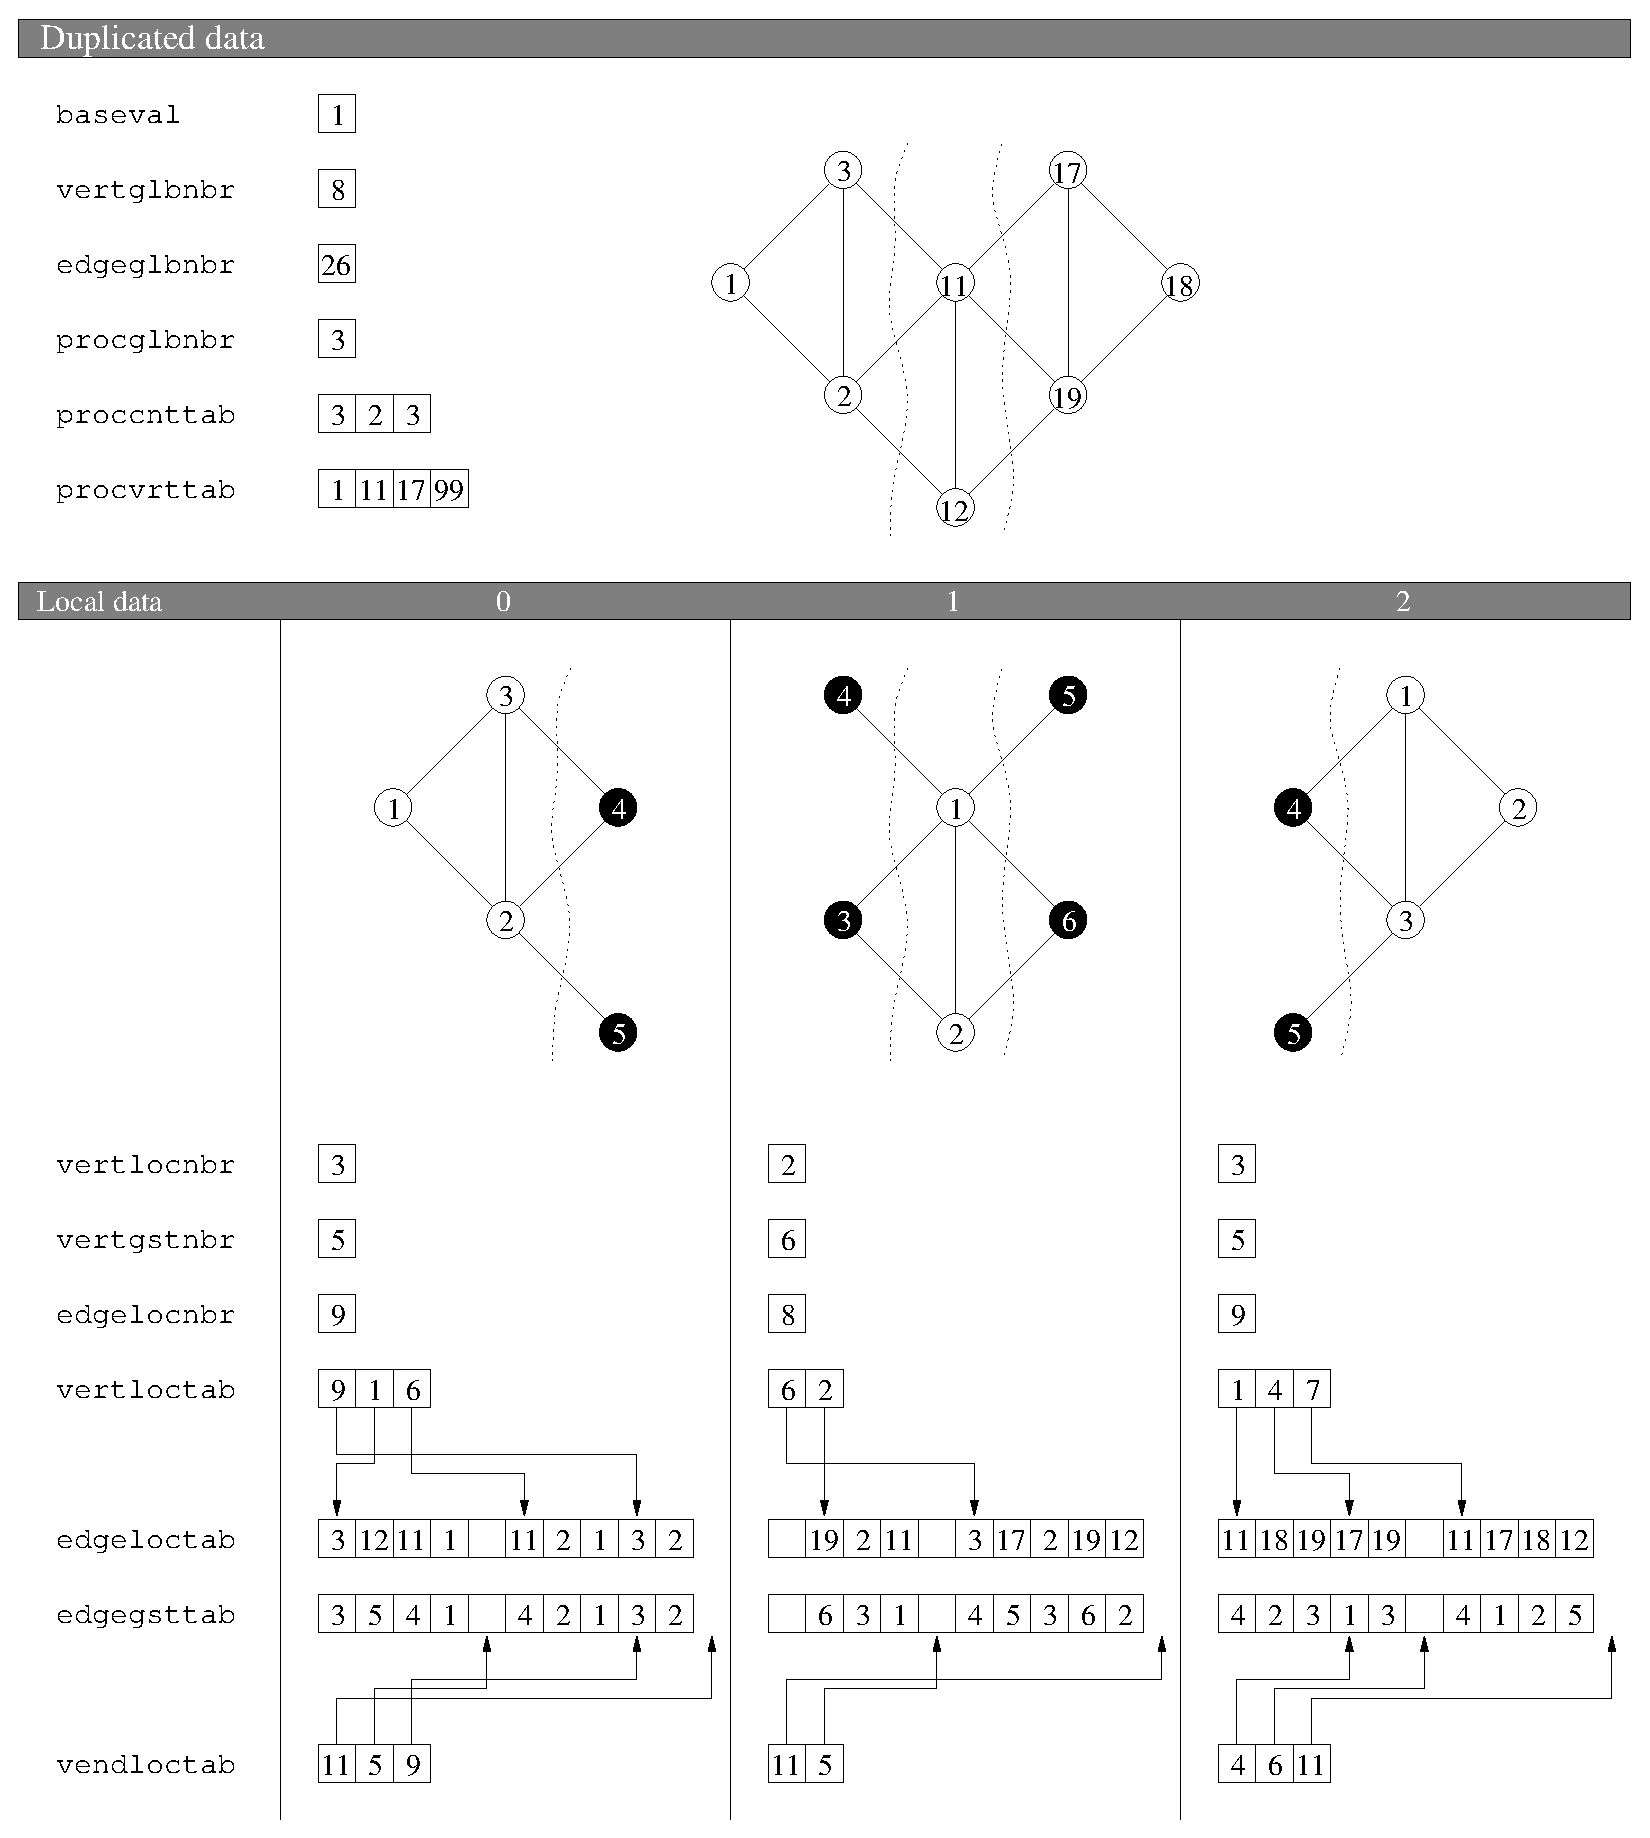
\includegraphics[scale=0.47]{p_f_gr2.eps}
\caption{Adjacency structure of the sample graph of
Figure~\protect\ref{fig-lib-dgraf-one} with a disjoint edge array and
a discontinuous ordering. Both {\tt vertloctab} and {\tt vendloctab}
are of size {\tt vertlocnbr}. This allows for the handling of dynamic
graphs, the structure of which can evolve with time.}
\label{fig-lib-dgraf-two}
\end{figure}

Dynamic graphs can be handled elegantly by using the
{\tt vend\lbt loc\lbt tab} and {\tt proc\lbt vrt\lbt tab} arrays.
In order to dynamically manage distributed graphs, one just has to
reserve index ranges large enough to create new vertices on each
process, and to allocate
{\tt vert\lbt loc\lbt tab}, {\tt vend\lbt loc\lbt tab} and
{\tt edge\lbt loc\lbt tab} arrays that are large
enough to contain all of the expected new vertex and edge
data. This can be done by passing {\tt SCOTCH\_\lbt graph\lbo Build} a
maximum number of local vertices, {\tt vert\lbt loc\lbt max}, greater
than the current number of local vertices, {\tt vert\lbt loc\lbt nbr}.

On every process $p$, vertices are globally labeled starting from
${\tt proc\lbt vrt\lbt tab}\mbox{\tt [}p\mbox{\tt ]}$, and locally
labeled from {\tt baseval}, leaving free space at the end of the local
arrays. To remove some vertex of local index $i$, one just has to
replace $\mbox{\tt vert\lbt loc\lbt tab}\mbox{\tt [}i\mbox{\tt ]}$ and
${\tt vend\lbt loc\lbt tab}\mbox{\tt [}i\mbox{\tt ]}$ with the values
of ${\tt vert\lbt loc\lbt tab}\lbt \mbox{\tt [vert\lbt loc\lbt
nbr}-1\mbox{\tt ]}$ and ${\tt vend\lbt loc\lbt tab}\lbt \mbox{\tt
[vert\lbt loc\lbt nbr}-1\mbox{\tt ]}$, respectively, and browse the
adjacencies of all neighbors of former vertex $(\mbox{\tt
vert}\lbt\mbox{\tt loc}\lbt\mbox{\tt nbr}-1)$ such that all
$(\mbox{\tt vert}\lbt\mbox{\tt loc}\lbt\mbox{\tt nbr}-1)$ indices are
turned into $i$s. Then, {\tt vert\lbt loc\lbt nbr} must be
decremented, and {\tt SCOTCH\_\lbt dgraph\lbt Build()} must be called
to account for the change of topology. If a graph building routine
such as {\tt SCOTCH\_\lbt dgraph\lbt Load()} or {\tt SCOTCH\_\lbt
dgraph\lbt Build()} had already been called on the {\tt SCOTCH\_\lbt
Dgraph} structure, {\tt SCOTCH\_\lbt dgraph\lbt Free()} has to be
called first in order to free the internal structures associated with
the older version of the graph, else these data would be lost, which
would result in memory leakage.

To add a new vertex, one has to fill {\tt vert\lbt loc\lbt tab\lbt
[vertnbr\lbt -1]} and {\tt vend\lbt loc\lbt tab\lbt [vertnbr\lbt -1]}
with the starting and end indices of the adjacency sub-array of the
new vertex. Then, the adjacencies of its neighbor vertices must also
be updated to account for it. If free space had been reserved at the
end of each of the neighbors, one just has to increment the
${\tt vend\lbt loc\lbt tab}\mbox{\tt [}i\mbox{\tt ]}$ values of every
neighbor $i$, and add the index of the new vertex at the end of the
adjacency sub-array. If the sub-array cannot be extended, then it has
to be copied elsewhere in the edge array, and both ${\tt vert\lbt
loc\lbt tab}\mbox{\tt [}i\mbox{\tt ]}$ and ${\tt vend\lbt loc\lbt
tab}\mbox{\tt [}i\mbox{\tt ]}$ must be updated accordingly. With
simple housekeeping of free areas of the edge array, dynamic arrays
can be updated with as little data movement as possible.

\subsubsection{Block ordering format}
\label{sec-lib-format-order}

Block orderings associated with distributed graphs are described by
means of block and permutation arrays, made of {\tt SCOTCH\_Num}s.  In
order for all orderings to have the same structure, irrespective of
whether they are centralized or distributed, or whether they are
created from graphs or meshes, all ordering data indices start from
{\tt baseval}. Consequently, row indices are related to vertex
indices in memory in the following way: row $i$ is associated with
vertex $i$ of the {\tt SCOTCH\_\lbt Dgraph} structure as if the vertex
numbering used for the graph was continuous.

Block orderings are made of the following data:
\begin{itemize}
\iteme[{\tt permtab}]
Array holding the permutation of the reordered matrix. Thus, if $k =
\mbox{\tt permtab}\mbox{\tt [}i\mbox{\tt ]}$, then row $i$ of the
original matrix is now row $k$ of the reordered matrix, that is, row
$i$ is the $k^{\mbox{th}}$ pivot.
\iteme[{\tt peritab}]
Inverse permutation of the reordered matrix. Thus, if $i = \mbox{\tt
peritab[$k$]}$, then row $k$ of the reordered matrix was row $i$ of
the original matrix.
\iteme[{\tt cblknbr}]
Number of column blocks (that is, supervariables) in the block ordering.
\iteme[{\tt rangtab}]
Array of ranges for the column blocks. Column block $c$, with
$\mbox{\tt baseval} \leq c < (\mbox{\tt cblknbr} + \mbox{\tt
baseval})$, contains columns with indices ranging from {\tt
rangtab[$i$]} to {\tt rangtab[$i + 1$]}, exclusive, in the reordered
matrix. Therefore,
{\tt rangtab[baseval]} is always equal to {\tt baseval}, and
{\tt rangtab[cblknbr + baseval]} is always equal to
$\mbox{\tt vert\lbt glb\lbt nbr} + \mbox{\tt baseval}$.
% for graphs
% and to $\mbox{\tt vnod\lbt glb\lbt nbr} + \mbox{\tt baseval}$ for meshes.
In order to avoid memory errors when column blocks are all single
columns, the size of {\tt rangtab} must always be one more than the
number of columns, that is, $\mbox{\tt vert\lbt glb\lbt nbr} + 1$.
% for graphs and $\mbox{\tt vnod\lbt glb\lbt nbr} + 1$ for meshes.
\iteme[{\tt treetab}]
Array of ascendants of permuted column blocks in the separators tree.
{\tt treetab[i]} is the index of the father of column block $i$ in the
separators tree, or $-1$ if column block $i$ is the root of the
separators tree. Whenever separators or leaves of the separators tree
are split into subblocks, as the block splitting, minimum fill or minimum
degree methods do, all subblocks of the same level are linked to the
column block of higher index belonging to the closest separator
ancestor. Indices in {\tt treetab} are based, in the same way as for
the other blocking structures. See Figure~\ref{fig-lib-ord-block} for
a complete example.
\end{itemize}

\begin{figure}
\centering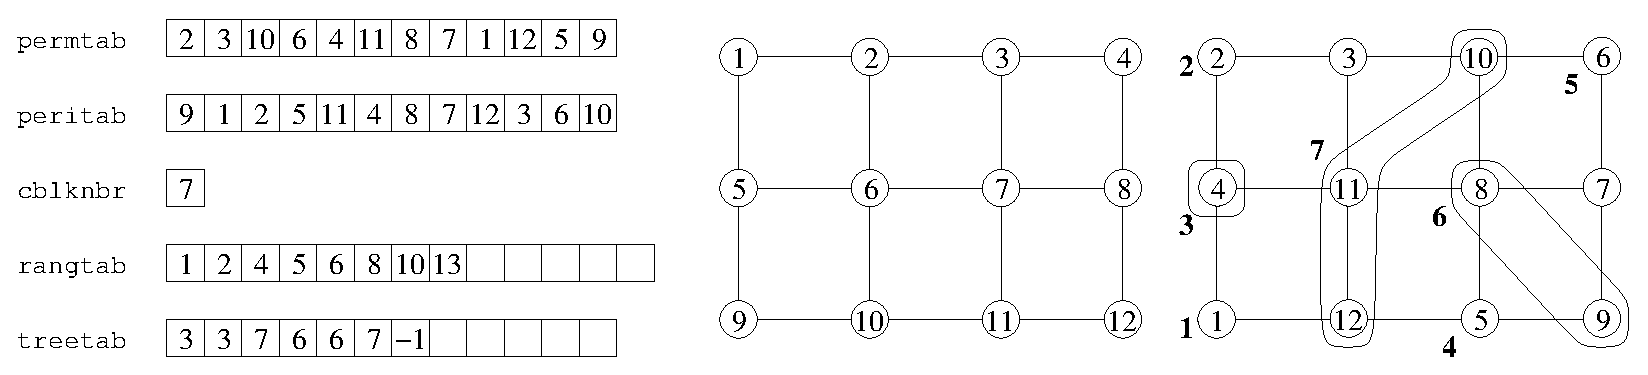
\includegraphics[scale=0.47]{p_f_orb.eps}
\caption{Arrays resulting from the ordering by complete nested
dissection of a 4 by 3 grid based from $1$. Leftmost grid is the
original grid, and righmost grid is the reordered grid, with
separators shown and column block indices written in bold.}
% using strategy  n{sep=hf{bal=0},ole=s,ose=s}
\label{fig-lib-ord-block}
\end{figure}

\subsection{Strategy strings}

The behavior of the static mapping and block ordering routines of the
\libscotch\ library is parametrized by means of strategy strings,
which describe how and when given partitioning or ordering methods
should be applied to graphs and subgraphs
% , or to meshes and submeshes.

\subsubsection{Using default strategy strings}
\label{sec-lib-format-strat-default}

While strategy strings can be built by hand, according to the syntax
given in the next sections, users who do not have specific needs can
take advantage of default strategies already implemented in the
\libscotch, which will yield very good results in most cases. By
doing so, they will spare themselves the hassle of updating their
strategies to comply to subsequent syntactic changes, and they will
benefit from the availability of new partitioning or ordering methods
as soon as they are made available.

The simplest way to use default strategy strings is to avoid
specifying any. By initializing a strategy object, by means of the
{\tt SCOTCH\_\lbt stratInit} routine, and by using the initialized
strategy object as is, without further parametrization, this object
will be filled with a default strategy when passing it as a parameter
to the next partitioning or ordering routine to be called. On return,
the strategy object will contain a fully specified strategy, tailored
for the type of operation which has been requested. Consequently, a
fresh strategy object that was used to partition a graph cannot be
used afterward as a default strategy for calling an ordering routine,
for instance, as partitioning and ordering strategies are incompatible.

The \libscotch\ also provides helper routines which allow users to
express their preferences on the kind of strategy that they
need. These helper routines, which are of the form
{\tt SCOTCH\_\lbt strat\lbt *\lbt Build}, tune default strategy strings
according to parameters provided by the user, such as the requested
number of parts (used as a hint to select the most efficient
partitioning routines), the desired maximum load imbalance ratio,
and a set of preference flags. While some of these flags are
antagonistic, most of them can be combined, by means of addition or
``binary or'' operators. These flags are the following.
They are grouped by application class.

\paragraph{Global flags}

\begin{itemize}
\iteme[{\tt SCOTCH\_STRATDEFAULT}]
Default behavior. No flags are set.
\iteme[{\tt SCOTCH\_STRATBALANCE}]
Enforce load balance as much as possible.
\iteme[{\tt SCOTCH\_STRATQUALITY}]
Privilege quality over speed.
\iteme[{\tt SCOTCH\_STRATSAFETY}]
Do not use methods that can lead to the occurrence of problematic
events, such as floating point exceptions, which could not be properly
handled by the calling software.
\iteme[{\tt SCOTCH\_STRATSPEED}]
Privilege speed over quality.
\end{itemize}

%% \paragraph{Mapping and partitioning flags}

%% \begin{itemize}
%% \iteme[{\tt SCOTCH\_STRATRECURSIVE}]
%% Use only recursive bipartitioning methods, and not direct k-way
%% methods. When this flag is not set, any combination of methods can be
%% used, so as to achieve the best result according to other user
%% preferences.
%% \iteme[{\tt SCOTCH\_STRATREMAP}]
%% Use the strategy for remapping an existing partition.
%% \end{itemize}

\paragraph{Ordering flags}

\begin{itemize}
\iteme[{\tt SCOTCH\_STRATLEVELMAX}]
Create at most the prescribed levels of nested dissection
separators. If the number of levels is less than the logarithm of the
number of processing elements used, distributed pieces of the
separated subgraph may have to be centralized so that the leaves can
be ordered, which may result in memory shortage.
\iteme[{\tt SCOTCH\_STRATLEVELMIN}]
Create at least the prescribed levels of nested dissection separators.
When used in conjunction with {\tt SCOTCH\_\lbt STRAT\lbt LEVEL\lbt
MAX}, the exact number of nested dissection levels will be performed,
unless the graph to order is too small.
\iteme[{\tt SCOTCH\_STRATLEAFSIMPLE}]
Order nested dissection leaves as cheaply as possible.
\iteme[{\tt SCOTCH\_STRATSEPASIMPLE}]
Order nested dissection separators as cheaply as possible.
\end{itemize}

\subsubsection{Parallel mapping strategy strings}
\label{sec-lib-format-pmap}

A parallel mapping strategy is made of one or several parallel
mapping methods, which can be combined by means of strategy
operators. The strategy operators that can be used in mapping
strategies are listed below, by increasing precedence.
\begin{itemize}
\iteme[{\tt (}{\it strat\/}{\tt )}]
Grouping operator.
The strategy enclosed within the parentheses is treated as a single
mapping method.
\iteme[{\tt /}{\it cond\/}{\tt ?}{\it strat1\/}{[{\tt :}{\it strat2}]{\tt ;}}]
Condition operator. According to the result of the evaluation of
condition {\it cond}, either {\it strat1\/} or {\it strat2\/} (if it
is present) is applied. The condition applies to the characteristics
of the current mapping task, and can be built from logical and
relational operators. Conditional operators are listed below, by
increasing precedence.
\begin{itemize}
\iteme[{\it cond1\/}{\tt |}{\it cond2}]
Logical or operator. The result of the condition is true if {\it cond1\/}
or {\it cond2\/} are true, or both.
\iteme[{\it cond1\/}{\tt \&}{\it cond2}]
Logical and operator. The result of the condition is true only if both
{\it cond1\/} and {\it cond2\/} are true.
\iteme[{\tt !}{\it cond}]
Logical not operator. The result of the condition is true only if
{\it cond\/} is false.
\iteme[{\it var} {\it relop} {\it val}]
Relational operator, where {\it var\/} is a node variable, {\it val\/} is
either a node variable or a constant of the type of variable {\it var}, and
{\it relop\/} is one of '{\tt\verb+<+}', '{\tt\verb+=+}', and '{\tt\verb+>+}'.
The node variables are listed below, along with their types.
\begin{itemize}
\iteme[{\tt edge}]
The global number of arcs of the current subgraph.
Integer.
\iteme[{\tt levl}]
The level of the subgraph in the recursion tree, starting from zero
for the initial graph at the root of the tree.
Integer.
\iteme[{\tt load}]
The overall sum of the vertex loads of the subgraph. It is equal to
{\tt vert} if the graph has no vertex loads.
Integer.
\iteme[{\tt mdeg}]
The maximum degree of the subgraph.
Integer.
\iteme[{\tt proc}]
The number of processes on which the current subgraph is distributed
at this level of the separators tree.
Integer.
\iteme[{\tt rank}]
The rank of the current process among the group of processes on
which the current subgraph is distributed at this level of the
separators tree.
Integer.
\iteme[{\tt vert}]
The global number of vertices of the current subgraph.
Integer.
\end{itemize}
\end{itemize}
\iteme[{\it method\/}{[{\tt \{}{\it parameters\/}{\tt \}}]}]
Parallel graph mapping method. Available parallel mapping methods
are listed below.
\end{itemize}
The currently available parallel mapping methods are the following.
\begin{itemize}
\iteme[{\tt r}]
Dual recursive bipartitioning method. The parameters of the dual recursive
bipartitioning method are given below.
\begin{itemize}
\iteme[{\tt seq=}{\it strat}]
Set the sequential mapping strategy that is used on every centralized
subgraph of the recursion tree, once the dual recursive bipartitioning
process has gone far enough such that the number of processes handling
some subgraph is restricted to one.
\iteme[{\tt sep=}{\it strat}]
Set the parallel graph bipartitioning strategy that is used on every
current job of the recursion tree. Parallel graph bipartitioning
strategies are described below, in section~\ref{sec-lib-format-pbipart}.
\end{itemize}
\end{itemize}

\subsubsection{Parallel graph bipartitioning strategy strings}
\label{sec-lib-format-pbipart}

A parallel graph bipartitioning strategy is made of one or several
parallel graph bipartitioning methods, which can be combined by means
of strategy operators. Strategy operators are listed below, by
increasing precedence.

\begin{itemize}
\iteme[{\it strat1\/}{\tt |}{\it strat2}]
Selection operator. The result of the selection is the best bipartition of
the two that are obtained by the distinct application of {\it strat1\/} and
{\it strat2\/} to the current bipartition.
\iteme[{\it strat1$\:$}{\it strat2}]
Combination operator. Strategy {\it strat2\/} is applied to the bipartition
resulting from the application of strategy {\it strat1\/} to the current
bipartition. Typically, the first method used should compute an initial
bipartition from scratch, and every following method should use the
result of the previous one at its starting point.
\iteme[{\tt (}{\it strat\/}{\tt )}]
Grouping operator.
The strategy enclosed within the parentheses is treated as a single
bipartitioning method.
\iteme[{\tt /}{\it cond\/}{\tt ?}{\it strat1\/}{[{\tt :}{\it strat2}]{\tt ;}}]
Condition operator. According to the result of the evaluation of condition
{\it cond}, either {\it strat1\/} or {\it strat2\/} (if it is present) is
applied. The condition applies to the characteristics of the current active
graph, and can be built from logical and relational operators. Conditional
operators are listed below, by increasing precedence.
\begin{itemize}
\iteme[{\it cond1\/}{\tt |}{\it cond2}]
Logical or operator. The result of the condition is true if {\it cond1\/}
or {\it cond2\/} are true, or both.
\iteme[{\it cond1\/}{\tt \&}{\it cond2}]
Logical and operator. The result of the condition is true only if both
{\it cond1\/} and {\it cond2\/} are true.
\iteme[{\tt !}{\it cond}]
Logical not operator. The result of the condition is true only if
{\it cond\/} is false.
\iteme[{\it var} {\it relop} {\it val}]
Relational operator, where {\it var\/} is a graph or node variable,
{\it val\/} is either a graph or node variable or a constant of the type of
variable {\it var\/}, and {\it relop\/} is one of
'{\tt\verb+<+}', '{\tt\verb+=+}', and '{\tt\verb+>+}'.
The graph and node variables are listed below, along with their types.
\begin{itemize}
\iteme[{\tt edge}]
The global number of edges of the current subgraph.
Integer.
\iteme[{\tt levl}]
The level of the subgraph in the bipartition or multi-level tree, starting from zero
for the initial graph at the root of the tree.
Integer.
\iteme[{\tt load}]
The overall sum of the vertex loads of the subgraph. It is equal to
{\tt vert} if the graph has no vertex loads.
Integer.
\iteme[{\tt load0}]
The vertex load of the first subset of the current bipartition of the current
graph.
Integer.
\iteme[{\tt proc}]
The number of processes on which the current subgraph is distributed
at this level of the nested dissection process.
Integer.
\iteme[{\tt rank}]
The rank of the current process among the group of processes on
which the current subgraph is distributed at this level of the
nested dissection process.
Integer.
\iteme[{\tt vert}]
The number of vertices of the current subgraph.
Integer.
\end{itemize}
\end{itemize}
The currently available parallel vertex separation methods are the
following.
\begin{itemize}
\iteme[{\tt b}]
Band method. Basing on the current distributed graph and on its
partition, this method creates a new distributed graph reduced to the
vertices which are at most at a given distance from the current
frontier, runs a parallel graph bipartitioning strategy on this graph,
and prolongs back the new bipartition to the current graph. This method
is primarily used to run bipartition refinement methods during the
uncoarsening phase of the multi-level parallel graph bipartitioning
method. The parameters of the band method are listed below.
\begin{itemize}
\iteme[{\tt bnd=}{\it strat}]
Set the parallel graph bipartitioning strategy to be applied to the band
graph.
\iteme[{\tt org=}{\it strat}]
Set the parallel graph bipartitioning strategy to be applied to the
full distributed graph if the band graph could not be extracted.
\iteme[{\tt width=}{\it val}]
Set the maximum distance from the current frontier of vertices to be
kept in the band graph. $0$ means that only frontier vertices
themselves are kept, $1$ that immediate neighboring vertices are kept
too, and so on.
\end{itemize}
\iteme[{\tt d}]
Parallel diffusion method. This method, presented in its sequential
formulation in~\cite{pell07b}, flows two kinds of antagonistic
liquids, scotch and anti-scotch, from two source vertices, and sets
the new frontier as the limit between vertices which contain scotch
and the ones which contain anti-scotch. Because selecting the source
vertices is essential to the obtainment of useful results, this method
has been hard-coded so that the two source vertices are the two
vertices of highest indices, since in the band method these are the
anchor vertices which represent all of the removed vertices of each
part. Therefore, this method must be used on band graphs only, or on
specifically crafted graphs. Applying it to any other graphs is very
likely to lead to extremely poor results.  The parameters of the
diffusion bipartitioning method are listed below.
\begin{itemize}
\iteme[{\tt dif=}{\it rat}]
Fraction of liquid which is diffused to neighbor vertices at each
pass. To achieve convergence, the sum of the {\tt dif} and {\tt rem}
parameters must be equal to $1$, but in order to speed-up the diffusion
process, other combinations of higher sum can be tried. In this case,
the number of passes must be kept low, to avoid numerical overflows
which would make the results useless.
\iteme[{\tt pass=}{\it nbr}]
Set the number of diffusion sweeps performed by the algorithm. This
number depends on the width of the band graph to which the diffusion
method is applied. Useful values range from $30$ to $500$ according
to chosen {\tt dif} and {\tt rem} coefficients.
\iteme[{\tt rem=}{\it rat}]
Fraction of liquid which remains on vertices at each pass. See above.
\end{itemize}
\iteme[{\tt m}]
Parallel multi-level method. The parameters of the multi-level method
are listed below.
\begin{itemize}
\iteme[{\tt asc=}{\it strat}]
Set the strategy that is used to refine the distributed bipartition
obtained at ascending levels of the uncoarsening phase by
prolongation of the bipartition computed for coarser graphs.
% or meshes.
This strategy is not applied to the coarsest graph,
% or mesh
for which only the {\tt low} strategy is used.
\iteme[{\tt dlevl=}{\it nbr}]
Set the minimum level after which duplication is allowed in the
folding process. A value of $-1$ results in duplication being always
performed when folding.
\iteme[{\tt dvert=}{\it nbr}]
Set the average number of vertices per process under which
the folding process is performed during the coarsening phase.
\iteme[{\tt low=}{\it strat}]
Set the strategy that is used to compute the bipartition of the
coarsest distributed graph,
% or mesh
at the lowest level of the coarsening process.
\iteme[{\tt rat=}{\it rat}]
Set the threshold maximum coarsening ratio over which graphs
% or meshes
are no longer coarsened. The ratio of any given coarsening cannot be
less that $0.5$ (case of a perfect matching), and cannot be greater
than $1.0$. Coarsening stops when either the coarsening ratio is
above the maximum coarsening ratio, or the graph
% or mesh
has fewer node vertices than the minimum number of vertices allowed.
\iteme[{\tt vert=}{\it nbr}]
Set the threshold minimum size under which graphs
% or meshes
are no longer coarsened. Coarsening stops when either the coarsening
ratio is above the maximum coarsening ratio, or the graph
% or mesh
has fewer node vertices than the minimum number of vertices allowed.
\end{itemize}
\iteme[{\tt q}]
Multi-sequential method. The current distributed graph and its
separator are centralized on every process that holds a part of it, and
a sequential graph bipartitioning method is applied independently to each
of them. Then, the best bipartition found is prolonged back to the
distributed graph. This method is primarily designed to operate on
band graphs, which are orders of magnitude smaller than their parent
graph. Else, memory bottlenecks are very likely to occur.
The parameters of the multi-sequential method are listed below.
\begin{itemize}
\iteme[{\tt strat=}{\it strat}]
Set the sequential edge separation strategy that is used to refine
the bipartition of the centralized graph. For a description of all of
the available sequential bipartitioning methods, please refer to the
{\it\scotch\ User's Guide}~\scotchcitesuser.
\end{itemize}
\iteme[{\tt x}]
Load balance enforcement method. This method moves as many vertices
from the heaviest part to the lightest one so as to reduce load
imbalance as much as possible, without impacting communication load
too negatively. The only parameter of this method is listed below.
\begin{itemize}
\iteme[{\tt sbbt=}{\it nbr}]
Number of sub-buckets to sort communication gains. $5$ is a common
value.
\end{itemize}
\iteme[{\tt z}]
Zero method. This method moves all of the vertices to the first
part, resulting in an empty frontier. Its main use is to stop the
bipartitioning process whenever some condition is true.
\end{itemize}
\end{itemize}

\subsubsection{Parallel ordering strategy strings}
\label{sec-lib-format-pord}

A parallel ordering strategy is made of one or several parallel
ordering methods, which can be combined by means of strategy
operators. The strategy operators that can be used in ordering
strategies are listed below, by increasing precedence.
\begin{itemize}
\iteme[{\tt (}{\it strat\/}{\tt )}]
Grouping operator.
The strategy enclosed within the parentheses is treated as a single
ordering method.
\iteme[{\tt /}{\it cond\/}{\tt ?}{\it strat1\/}{[{\tt :}{\it strat2}]{\tt ;}}]
Condition operator. According to the result of the evaluation of
condition {\it cond}, either {\it strat1\/} or {\it strat2\/} (if it
is present) is applied. The condition applies to the characteristics
of the current node of the separators tree, and can be built from
logical and relational operators. Conditional operators are listed
below, by increasing precedence.
\begin{itemize}
\iteme[{\it cond1\/}{\tt |}{\it cond2}]
Logical or operator. The result of the condition is true if {\it cond1\/}
or {\it cond2\/} are true, or both.
\iteme[{\it cond1\/}{\tt \&}{\it cond2}]
Logical and operator. The result of the condition is true only if both
{\it cond1\/} and {\it cond2\/} are true.
\iteme[{\tt !}{\it cond}]
Logical not operator. The result of the condition is true only if
{\it cond\/} is false.
\iteme[{\it var} {\it relop} {\it val}]
Relational operator, where {\it var\/} is a node variable, {\it val\/} is
either a node variable or a constant of the type of variable {\it var}, and
{\it relop\/} is one of '{\tt\verb+<+}', '{\tt\verb+=+}', and '{\tt\verb+>+}'.
The node variables are listed below, along with their types.
\begin{itemize}
\iteme[{\tt edge}]
The global number of arcs of the current subgraph.
Integer.
\iteme[{\tt levl}]
The level of the subgraph in the separators tree, starting from zero
for the initial graph at the root of the tree.
Integer.
\iteme[{\tt load}]
The overall sum of the vertex loads of the subgraph. It is equal to
{\tt vert} if the graph has no vertex loads.
Integer.
\iteme[{\tt mdeg}]
The maximum degree of the subgraph.
Integer.
\iteme[{\tt proc}]
The number of processes on which the current subgraph is distributed
at this level of the separators tree.
Integer.
\iteme[{\tt rank}]
The rank of the current process among the group of processes on
which the current subgraph is distributed at this level of the
separators tree.
Integer.
\iteme[{\tt vert}]
The global number of vertices of the current subgraph.
Integer.
\end{itemize}
\end{itemize}
\iteme[{\it method\/}{[{\tt \{}{\it parameters\/}{\tt \}}]}]
Parallel graph ordering method. Available parallel ordering methods
are listed below.
\end{itemize}
The currently available parallel ordering methods are the following.
\begin{itemize}
\iteme[{\tt n}]
Nested dissection method. The parameters of the nested dissection
method are given below.
\begin{itemize}
\iteme[{\tt ole=}{\it strat}]
Set the parallel ordering strategy that is used on every distributed
leaf of the parallel separators tree if the node separation strategy
{\tt sep} has failed to separate it further.
\iteme[{\tt ose=}{\it strat}]
Set the parallel ordering strategy that is used on every distributed
separator of the separators tree.
\iteme[{\tt osq=}{\it strat}]
Set the sequential ordering strategy that is used on every centralized
subgraph of the separators tree, once the nested dissection process has
gone far enough such that the number of processes handling some
subgraph is restricted to one.
\iteme[{\tt sep=}{\it strat}]
Set the parallel node separation strategy that is used on every
current leaf of the separators tree to make it grow. Parallel
node separation strategies are described below, in
section~\ref{sec-lib-format-pnsep}.
\end{itemize}
\iteme[{\tt q}]
Sequential ordering method. The distributed graph is gathered onto a
single process which runs a sequential ordering strategy. The only
parameter of the sequential method is given below.
\begin{itemize}
\iteme[{\tt strat=}{\it strat}]
Set the sequential ordering strategy that is applied to the
centralized graph. For a description of all of the available
sequential ordering methods, please refer to the
{\it\scotch\ User's Guide}~\scotchcitesuser.
\end{itemize}
\iteme[{\tt s}]
Simple method. Vertices are ordered in their natural order. This
method is fast, and should be used to order separators if the number
of extra-diagonal blocks is not relevant
\end{itemize}

\subsubsection{Parallel node separation strategy strings}
\label{sec-lib-format-pnsep}

A parallel node separation strategy is made of one or several parallel
node separation methods, which can be combined by means of strategy
operators. Strategy operators are listed below, by increasing
precedence.

\begin{itemize}
\iteme[{\it strat1\/}{\tt |}{\it strat2}]
Selection operator. The result of the selection is the best vertex separator of
the two that are obtained by the distinct application of {\it strat1\/} and
{\it strat2\/} to the current separator.
\iteme[{\it strat1$\:$}{\it strat2}]
Combination operator. Strategy {\it strat2\/} is applied to the vertex
separator resulting from the application of strategy {\it strat1\/} to the
current separator. Typically, the first method used should compute an initial
separation from scratch, and every following method should use the
result of the previous one as a starting point.
\iteme[{\tt (}{\it strat\/}{\tt )}]
Grouping operator.
The strategy enclosed within the parentheses is treated as a single
separation method.
\iteme[{\tt /}{\it cond\/}{\tt ?}{\it strat1\/}{[{\tt :}{\it strat2}]{\tt ;}}]
Condition operator. According to the result of the evaluation of condition
{\it cond}, either {\it strat1\/} or {\it strat2\/} (if it is present) is
applied. The condition applies to the characteristics of the current subgraph,
and can be built from logical and relational operators. Conditional
operators are listed below, by increasing precedence.
\begin{itemize}
\iteme[{\it cond1\/}{\tt |}{\it cond2}]
Logical or operator. The result of the condition is true if {\it cond1\/}
or {\it cond2\/} are true, or both.
\iteme[{\it cond1\/}{\tt \&}{\it cond2}]
Logical and operator. The result of the condition is true only if both
{\it cond1\/} and {\it cond2\/} are true.
\iteme[{\tt !}{\it cond}]
Logical not operator. The result of the condition is true only if
{\it cond\/} is false.
\iteme[{\it var} {\it relop} {\it val}]
Relational operator, where {\it var\/} is a graph or node variable,
{\it val\/} is either a graph or node variable or a constant of the type of
variable {\it var\/}, and {\it relop\/} is one of
'{\tt\verb+<+}', '{\tt\verb+=+}', and '{\tt\verb+>+}'.
The graph and node variables are listed below, along with their types.
\begin{itemize}
\iteme[{\tt edge}]
The global number of edges of the current subgraph.
Integer.
\iteme[{\tt levl}]
The level of the subgraph in the separators tree, starting from zero
for the initial graph at the root of the tree.
Integer.
\iteme[{\tt load}]
The overall sum of the vertex loads of the subgraph. It is equal to
{\tt vert} if the graph has no vertex loads.
Integer.
\iteme[{\tt proc}]
The number of processes on which the current subgraph is distributed
at this level of the nested dissection process.
Integer.
\iteme[{\tt rank}]
The rank of the current process among the group of processes on
which the current subgraph is distributed at this level of the
nested dissection process.
Integer.
\iteme[{\tt vert}]
The number of vertices of the current subgraph.
Integer.
\end{itemize}
\end{itemize}
The currently available parallel vertex separation methods are the
following.
\begin{itemize}
\iteme[{\tt b}]
Band method. Basing on the current distributed graph and on its
partition, this method creates a new distributed graph reduced to the
vertices which are at most at a given distance from the current
separator, runs a parallel vertex separation strategy on this graph,
and prolongs back the new separator to the current graph. This method
is primarily used to run separator refinement methods during the
uncoarsening phase of the multi-level parallel graph separation
method. The parameters of the band method are listed below.
\begin{itemize}
\iteme[{\tt strat=}{\it strat}]
Set the parallel vertex separation strategy to be applied to the band
graph.
\iteme[{\tt width=}{\it val}]
Set the maximum distance from the current separator of vertices to be
kept in the band graph. $0$ means that only separator vertices
themselves are kept, $1$ that immediate neighboring vertices are kept
too, and so on.
\end{itemize}
\iteme[{\tt m}]
Parallel vertex multi-level method. The parameters of the vertex
multi-level method are listed below.
\begin{itemize}
\iteme[{\tt asc=}{\it strat}]
Set the strategy that is used to refine the distributed vertex
separators obtained at ascending levels of the uncoarsening phase by
prolongation of the separators computed for coarser graphs.
% or meshes.
This strategy is not applied to the coarsest graph,
% or mesh
for which only the {\tt low} strategy is used.
\iteme[{\tt dlevl=}{\it nbr}]
Set the minimum level after which duplication is allowed in the
folding process. A value of $-1$ results in duplication being always
performed when folding.
\iteme[{\tt dvert=}{\it nbr}]
Set the average number of vertices per process under which
the folding process is performed during the coarsening phase.
\iteme[{\tt low=}{\it strat}]
Set the strategy that is used to compute the vertex separator of the
coarsest distributed graph,
% or mesh
at the lowest level of the coarsening process.
\iteme[{\tt rat=}{\it rat}]
Set the threshold maximum coarsening ratio over which graphs
% or meshes
are no longer coarsened. The ratio of any given coarsening cannot be
less that $0.5$ (case of a perfect matching), and cannot be greater
than $1.0$. Coarsening stops when either the coarsening ratio is
above the maximum coarsening ratio, or the graph
% or mesh
has fewer node vertices than the minimum number of vertices allowed.
\iteme[{\tt vert=}{\it nbr}]
Set the threshold minimum size under which graphs
% or meshes
are no longer coarsened. Coarsening stops when either the coarsening
ratio is above the maximum coarsening ratio, or the graph
% or mesh
has fewer node vertices than the minimum number of vertices allowed.
\end{itemize}
\iteme[{\tt q}]
Multi-sequential method. The current distributed graph and its
separator are centralized on every process that holds a part of it, and
a sequential vertex separation method is applied independently to each
of them. Then, the best separator found is prolonged back to the
distributed graph. This method is primarily designed to operate on
band graphs, which are orders of magnitude smaller than their parent
graph. Else, memory bottlenecks are very likely to occur.
The parameters of the multi-sequential method are listed below.
\begin{itemize}
\iteme[{\tt strat=}{\it strat}]
Set the sequential vertex separation strategy that is used to refine
the separator of the centralized graph. For a description of all of
the available sequential methods, please refer to the
{\it\scotch\ User's Guide}~\scotchcitesuser.
\end{itemize}
\iteme[{\tt z}]
Zero method. This method moves all of the node vertices to the first
part, resulting in an empty separator. Its main use is to stop the
separation process whenever some condition is true.
\end{itemize}
\end{itemize}

\subsection{Distributed graph handling routines}
\label{sec-lib-dgraph}

\subsubsection{{\tt SCOTCH\_dgraphAlloc}}

\begin{itemize}
\progsyn

{\tt\begin{tabular}{l@{}l}
SCOTCH\_Dgraph * SCOTCH\_dgraphAlloc ( & void)
\end{tabular}}

\progdes

The {\tt SCOTCH\_dgraphAlloc} function allocates a memory area of a
size sufficient to store a {\tt SCOTCH\_\lbt Dgraph} structure. It is
the user's responsibility to free this memory when it is no longer
needed. The allocated space must be initialized before use, by means
of the {\tt SCOTCH\_\lbt dgraph\lbt Init} routine.

\progret

{\tt SCOTCH\_dgraphAlloc} returns the pointer to the memory area if it
has been successfully allocated, and {\tt NULL} else.
\end{itemize}

\subsubsection{{\tt SCOTCH\_dgraphBand}}

\begin{itemize}
\progsyn

{\tt\begin{tabular}{l@{}ll}
int SCOTCH\_dgraphBand ( & SCOTCH\_Dgraph * const    & orggrafptr, \\
                         & const SCOTCH\_Num         & fronlocnbr, \\
                         & const SCOTCH\_Num * const & fronloctab, \\
                         & const SCOTCH\_Num         & distval,    \\
                         & SCOTCH\_Dgraph * const    & bndgrafptr) \\
\end{tabular}}

{\tt\begin{tabular}{l@{}ll}
scotchfdgraphband ( & doubleprecision (*)   & orggrafdat, \\
                    & integer*{\it num}     & seedlocnbr, \\
                    & integer*{\it num} (*) & seedloctab, \\
                    & integer*{\it num}     & distval,    \\
                    & doubleprecision (*)   & bndgrafdat, \\
                    & integer               & ierr)
\end{tabular}}

\progdes

The {\tt SCOTCH\_dgraphBand} routine creates in the {\tt SCOTCH\_\lbt
Dgraph} structure pointed to by {\tt bndgrafptr} a distributed band
graph induced from the {\tt SCOTCH\_\lbt Dgraph} pointed to by {\tt
orggrafptr}. The distributed band graph will contain all the vertices
of the original graph located at a distance smaller than or equal to
{\tt distval} from any vertex provided in the {\tt seedloctab} lists
of seed vertices.

On each process, the {\tt seedloctab} array should contain the local
indices of the local vertices that will serve as seeds. The number of
such local vertices is passed to {\tt SCOTCH\_\lbt dgraph\lbt Band} in
the {\tt seedlocnbr} value. The size of the {\tt seedloctab} array
should be at least equal to the number of local vertices of the
original graph, as it is internally used as a queue array. Hence, no
user data should be placed immediately after the {\tt seedlocnbr}
values in the array, as they are most likely to be overwritten by
{\tt SCOTCH\_\lbt dgraph\lbt Band}.

{\tt bndgrafptr} must have been initialized with the
{\tt SCOTCH\_\lbt dgraph\lbt Init} routine before
{\tt SCOTCH\_dgraph\lbt Band} is called. The communicator that is
passed to it can either be the communicator used by the original graph
{\tt org\lbt graf\lbt ptr}, or any congruent communicator created by
using {\tt MPI\_\lbt Comm\_\lbt dup} on this communicator. Using a
distinct communicator for the induced band graph allows subsequent
library routines to be called in parallel on the two graphs after the
band graph is created.

Induced band graphs have vertex labels attached to each of their
vertices, in the {\tt vlbl\lbt loc\lbt tab} array. If the original
graph had vertex labels attached to it, band graph vertex labels are
the labels of the corresponding vertices in the original graph. Else,
band graph vertex labels are the global indices of corresponding
vertices in the original graph.

Depending on original graph vertex and seed distributions, the
distribution of induced band graph vertices may be highly
imbalanced. In order for further computations on this distributed
graph to scale well, a redistribution of its data may be necessary,
using the {\tt SCOTCH\_dgraph\lbt Redist} routine.

\progret

{\tt SCOTCH\_dgraphBand} returns $0$ if the band graph structure has
been successfully created, and $1$ else.
\end{itemize}

\subsubsection{{\tt SCOTCH\_dgraphBuild}}

\begin{itemize}
\progsyn

{\tt\begin{tabular}{l@{}ll}
int SCOTCH\_dgraphBuild ( & SCOTCH\_Dgraph *    & grafptr,    \\
                          & const SCOTCH\_Num   & baseval,    \\
                          & const SCOTCH\_Num   & vertlocnbr, \\
                          & const SCOTCH\_Num   & vertlocmax, \\
                          & const SCOTCH\_Num * & vertloctab, \\
                          & const SCOTCH\_Num * & vendloctab, \\
                          & const SCOTCH\_Num * & veloloctab, \\
                          & const SCOTCH\_Num * & vlblocltab, \\
                          & const SCOTCH\_Num   & edgelocnbr, \\
                          & const SCOTCH\_Num   & edgelocsiz, \\
                          & const SCOTCH\_Num * & edgeloctab, \\
                          & const SCOTCH\_Num * & edgegsttab, \\
                          & const SCOTCH\_Num * & edloloctab)
\end{tabular}}

{\tt\begin{tabular}{l@{}ll}
scotchfdgraphbuild ( & doubleprecision (*)   & grafdat,    \\
                     & integer*{\it num}     & baseval,    \\
                     & integer*{\it num}     & vertlocnbr, \\
                     & integer*{\it num}     & vertlocmax, \\
                     & integer*{\it num} (*) & vertloctab, \\
                     & integer*{\it num} (*) & vendloctab, \\
                     & integer*{\it num} (*) & veloloctab, \\
                     & integer*{\it num} (*) & vlblloctab, \\
                     & integer*{\it num}     & edgelocnbr, \\
                     & integer*{\it num}     & edgelocsiz, \\
                     & integer*{\it num} (*) & edgeloctab, \\
                     & integer*{\it num} (*) & edgegsttab, \\
                     & integer*{\it num} (*) & edloloctab, \\
                     & integer               & ierr)
\end{tabular}}

\progdes

The {\tt SCOTCH\_dgraphBuild} routine fills the distributed source
graph structure pointed to by {\tt grafptr} with all of the data that
are passed to it.

{\tt baseval} is the graph base value for index arrays (typically $0$ for
structures built from C and $1$ for structures built from Fortran).
{\tt vertlocnbr} is the number of local vertices on the calling
process, used to create the {\tt proccnttab} array.
{\tt vertlocmax} is the maximum number of local vertices to be created
on the calling process, used to create the {\tt proc\lbt vrt\lbt tab}
array of global indices, and which must be set to {\tt vert\lbt
loc\lbt nbr} for graphs wihout holes in their global numbering.
{\tt vertloctab} is the local adjacency index array, of size $({\tt
vertlocnbr} + 1)$ if the edge array is compact (that is, if {\tt
vendloctab} equals $\mbox{\tt vertloctab}+1$ or {\tt NULL}), or of
size {\tt vertlocnbr} else.
{\tt vendloctab} is the adjacency end index array, of size {\tt
vertlocnbr} if it is disjoint from {\tt vertloctab}.
{\tt veloloctab} is the local vertex load array, of size
{\tt vertlocnbr} if it exists.
{\tt vlblloctab} is the local vertex label array, of size
{\tt vertlocnbr} if it exists.
{\tt edgelocnbr} is the local number of arcs (that is, twice the
number of edges), including arcs to local vertices as well as to
ghost vertices.
{\tt edgelocsiz} is lower-bounded by the minimum size of the edge
array required to encompass all used adjacency values; it is therefore
at least equal to the maximum of the {\tt vendloctab} entries, over
all local vertices, minus {\tt baseval}; it can be set to {\tt
edgelocnbr} if the edge array is compact.
{\tt edgeloctab} is the local adjacency array, of size at least
{\tt edgelocsiz}, which stores the global indices of end vertices.
{\tt edgegsttab} is the adjacency array, of size at least
{\tt edgelocsiz}, if it exists; if {\tt edgegsttab} is given, it is
assumed to be a pointer to an empty array to be filled with ghost
vertex data computed by {\tt SCOTCH\_dgraph\lbt Ghst} whenever
needed by communication routines such as
{\tt SCOTCH\_dgraph\lbt Halo}.
{\tt edloloctab} is the arc load array, of size {\tt edgelocsiz}
if it exists.

The {\tt vendloctab}, {\tt veloloctab}, {\tt vlblloctab},
{\tt edloloctab} and {\tt edgegsttab} arrays are optional,
and a null pointer can be passed as argument whenever
they are not defined.

Note that, for \ptscotch\ to operate properly, either all the arrays
of a kind must be set to null on all processes, or else all of them
must be non null. This is mandatory because some algorithms require that
collective communication operations be performed when some kind of
data is present. If some processes considered that the arrays are
present, and start such communications, while others did not, a
deadlock would occur. In most cases, this situation will be
anticipated and an error message will be issued, stating that graph
data are inconsistent.

The situation above may accidentally arise when some processes don't
own any edge or vertex. In that case, depending on the implementation,
a user \texttt{malloc} of size zero may return a null pointer rather
than a non null pointer to an area of size zero, leading to the
aforementioned inconsistencies. In order to avoid this problem, it is
necessary to ensure that no null pointer will be returned, even in the
case when zero bytes are requested. A workaround can be to call
\texttt{malloc (\textit{x} | 4)} instead of \texttt{malloc
(\textit{x})}. The ``\texttt{| 4}'' will consume only $4$ extra bytes
at most, depending on the value of \texttt{\textit{x}}.

Since, in Fortran, there is no null reference, passing the
{\tt scotchf\lbt dgraph\lbt build} routine a reference equal to
{\tt vertloctab} in the {\tt veloloctab} or {\tt vlblloctab} fields
makes them be considered as missing arrays. The same holds for
{\tt edloloctab} and {\tt edgegsttab} when they are passed a
reference equal to {\tt edgeloctab}. Setting {\tt vendloctab}
to refer to one cell after {\tt vertloctab} yields the same result,
as it is the exact semantics of a compact vertex array.

To limit memory consumption, {\tt SCOTCH\_\lbt dgraph\lbo Build} does
not copy array data, but instead references them in the {\tt
SCOTCH\_\lbt Dgraph} structure. Therefore, great care should be taken
not to modify the contents of the arrays passed to {\tt SCOTCH\_\lbt
dgraph\lbo Build} as long as the graph structure is in use. Every
update of the arrays should be preceded by a call to {\tt SCOTCH\_\lbt
dgraph\lbo Free}, to free internal graph structures, and eventually
followed by a new call to {\tt SCOTCH\_\lbt dgraph\lbo Build} to
re-build these internal structures so as to be able to use the new
distributed graph.

To ensure that inconsistencies in user data do not result in an
erroneous behavior of the \libscotch\ routines, it is recommended, at
least in the development stage of your application code, to call the
{\tt SCOTCH\_\lbt dgraph\lbt Check} routine on the newly created
{\tt SCOTCH\_\lbt Dgraph} structure before calling any other
\libscotch\ routine.

\progret

{\tt SCOTCH\_dgraphBuild} returns $0$ if the graph structure has been
successfully set with all of the input data, and $1$ else.
\end{itemize}

\subsubsection{{\tt SCOTCH\_dgraphCheck}}

\begin{itemize}
\progsyn

{\tt\begin{tabular}{l@{}ll}
int SCOTCH\_dgraphCheck ( & const SCOTCH\_Dgraph * & grafptr)
\end{tabular}}

{\tt\begin{tabular}{l@{}ll}
scotchfdgraphcheck ( & doubleprecision (*) & grafdat, \\
                     & integer             & ierr)
\end{tabular}}

\progdes

The {\tt SCOTCH\_dgraphCheck} routine checks the consistency of the
given {\tt SCOTCH\_\lbt Dgraph} structure. It can be used in client
applications to determine if a graph which has been created from
user-generated data by means of the {\tt SCOTCH\_\lbt dgraph\lbt Build}
routine is consistent, prior to calling any other routines of the
\libscotch\ library which would otherwise return internal error
messages or crash the program.

\progret

{\tt SCOTCH\_dgraphCheck} returns $0$ if graph data are consistent, and
$1$ else.

\end{itemize}

\subsubsection{{\tt SCOTCH\_dgraphCoarsen}}

\begin{itemize}
\progsyn

{\tt\begin{tabular}{l@{}ll}
int SCOTCH\_dgraphCoarsen ( & SCOTCH\_Dgraph * const & finegrafptr, \\
                            & const SCOTCH\_Num      & coarnbr,     \\
                            & const double           & coarrat,     \\
                            & const SCOTCH\_Num      & flagval,     \\
                            & SCOTCH\_Dgraph * const & coargrafptr, \\
                            & SCOTCH\_Num * const    & multloctab)  \\
\end{tabular}}

{\tt\begin{tabular}{l@{}ll}
scotchfdgraphcoarsen ( & doubleprecision (*)   & finegrafdat, \\
                       & integer*{\it num}     & coarnbr,     \\
                       & doubleprecision       & coarrat,     \\
                       & integer*{\it num}     & flagval,     \\
                       & doubleprecision (*)   & coargrafdat, \\
                       & integer*{\it num} (*) & multloctab,  \\
                       & integer               & ierr)
\end{tabular}}

\progdes

The {\tt SCOTCH\_dgraphCoarsen} routine creates in the
{\tt SCOTCH\_\lbt Dgraph} structure pointed to by {\tt coargrafptr}
a distributed coarsened graph from the {\tt SCOTCH\_\lbt Dgraph}
pointed to by {\tt finegrafptr}. The coarsened graph is created only
if it is comprises more than {\tt coarnbr} vertices, or if the
coarsening ratio is lower than {\tt coarrat}. Valid coarsening ratio
values range from $0.5$ (in the case of a perfect matching) to $1.0$
(if no vertex could be coarsened). Classical threshold values range
from $0.7$ to $0.8$.

The {\tt flagval} flag specifies the type of coarsening. Several
groups of flags can be combined, by means of addition or
``binary or'' operators. When {\tt SCOTCH\_\lbt COARSEN\lbt
NO\lbt MERGE} is set, isolated vertices are never merged with other
vertices. This preserves the topology of the graph, at the expense of
a higher coarsening ratio. When {\tt SCOTCH\_\lbt COARSEN\lbt
FOLD} or {\tt SCOTCH\_\lbt COARSEN\lbt FOLD\lbt DUP} are set, if a
coarsened graph is created, it is folded onto half of the processes of
the initial communicator. In the case of {\tt SCOTCH\_\lbt COARSEN\lbt
FOLD\lbt DUP}, a second copy is created (duplicated) onto the other
half. The two copies may not be identical, if the number of processors
of the finer graph is odd.

The {\tt multloctab} array must be of a size that is big enough to
store multinode data for the resulting coarsened graph. This array
will contain pairs of consecutive {\tt SCOTCH\_\lbt Num} values,
representing the global indices of the two fine vertices that have
been coarsened into each of the local coarse vertices. In case of
plain coarsening, the size of the array must be at least twice the
maximum expected number of local coarse vertices, that is, on each
processor, twice the value of {\tt vert\lbt loc\lbt nbr} of the finer
graph, because in the worst case no coarsening may happen on some
processor. In case of folding, a redistribution of vertices is
performed. Hence, the maximum number of coarse vertices on some
processor is upper-bounded by the expected maximum global number of
coarse vertices, divided by the resulting number of processors, that
is, the integer floor value of half of the number of processors of the
finer graph.

{\tt coargrafptr} must have been initialized with the
{\tt SCOTCH\_\lbt dgraph\lbt Init} routine before
{\tt SCOTCH\_dgraph\lbt Coarsen} is called. The communicator that is
passed to it can either be the communicator used by the fine graph
{\tt fine\lbt graf\lbt ptr}, or any congruent communicator created by
using {\tt MPI\_\lbt Comm\_\lbt dup} on this communicator. Using a
distinct communicator for the coarsened subgraph allows subsequent
library routines to be called in parallel on the two graphs after the
coarse graph is created.

Depending on the way vertex mating is performed, the distribution of
coarsened graph vertices may be imbalanced. In order for further
computations on this distributed graph to scale well, a redistribution
of its data might be necessary, using the
{\tt SCOTCH\_dgraph\lbt Redist} routine.

\progret

{\tt SCOTCH\_dgraphCoarsen} returns $0$ if the coarse graph
structure has been successfully created, $1$ if the coarse graph was
not created because it did not enforce the threshold parameters, and
$2$ on error.
\end{itemize}

\subsubsection{{\tt SCOTCH\_dgraphData}}
\label{sec-lib-func-scotchdgraphdata}

\begin{itemize}
\progsyn

{\tt\begin{tabular}{l@{}ll}
void SCOTCH\_dgraphData ( & const SCOTCH\_Graph * & grafptr,    \\
                          & SCOTCH\_Num *         & baseptr,    \\
                          & SCOTCH\_Num *         & vertglbptr, \\
                          & SCOTCH\_Num *         & vertlocptr, \\
                          & SCOTCH\_Num *         & vertlocptz, \\
                          & SCOTCH\_Num *         & vertgstptr, \\
                          & SCOTCH\_Num **        & vertloctab, \\
                          & SCOTCH\_Num **        & vendloctab, \\
                          & SCOTCH\_Num **        & veloloctab, \\
                          & SCOTCH\_Num **        & vlblloctab, \\
                          & SCOTCH\_Num *         & edgeglbptr, \\
                          & SCOTCH\_Num *         & edgelocptr, \\
                          & SCOTCH\_Num *         & edgelocptz, \\
                          & SCOTCH\_Num **        & edgeloctab, \\
                          & SCOTCH\_Num **        & edgegsttab, \\
                          & SCOTCH\_Num **        & edloloctab, \\
                          & MPI\_Comm *           & comm)
\end{tabular}}

{\tt\begin{tabular}{l@{}ll}
scotchfdgraphdata ( & doubleprecision (*)   & grafdat,    \\
                    & integer*{\it num} (*) & indxtab,    \\
                    & integer*{\it num}     & baseval,    \\
                    & integer*{\it num}     & vertglbnbr, \\
                    & integer*{\it num}     & vertlocnbr, \\
                    & integer*{\it num}     & vertlocmax, \\
                    & integer*{\it num}     & vertgstnbr, \\
                    & integer*{\it idx}     & vertlocidx, \\
                    & integer*{\it idx}     & vendlocidx, \\
                    & integer*{\it idx}     & velolocidx, \\
                    & integer*{\it idx}     & vlbllocidx, \\
                    & integer*{\it num}     & edgeglbnbr, \\
                    & integer*{\it num}     & edgelocnbr, \\
                    & integer*{\it num}     & edgelocsiz, \\
                    & integer*{\it idx}     & edgelocidx, \\
                    & integer*{\it idx}     & edgegstidx, \\
                    & integer*{\it idx}     & edlolocidx, \\
                    & integer               & comm)
\end{tabular}}

\progdes

The {\tt SCOTCH\_dgraphData} routine is the dual of the
{\tt SCOTCH\_\lbt dgraph\lbo Build} routine. It is a multiple
accessor that returns scalar values and array references.

{\tt baseptr} is the pointer to a location that will hold the graph base
value for index arrays (typically $0$ for
structures built from C and $1$ for structures built from Fortran).
{\tt vertglbptr} is the pointer to a location that will hold the
global number of vertices.
{\tt vertlocptr} is the pointer to a location that will hold the
number of local vertices.
{\tt vertlocptz} is the pointer to a location that will hold the
maximum allowed number of local vertices, that is,
$(\mbox{\tt proc\lbt vrt\lbt tab[}p + 1\mbox{\tt]} -
\mbox{\tt proc\lbt vrt\lbt tab[}p\mbox{\tt]})$, where $p$ is the
rank of the local process.
{\tt vertgstptr} is the pointer to a location that will hold the
number of local and ghost vertices if it has already been computed
by a prior call to {\tt SCOTCH\_\lbt dgraph\lbo Ghst}, and $-1$ else.
{\tt vertloctab} is the pointer to a location that will hold the
reference to the adjacency index array, of size
$\mbox{\tt *vertlocptr} + 1$ if the adjacency array is compact,
or of size {\tt *vertlocptr} else.
{\tt vendloctab} is the pointer to a location that will hold the
reference to the adjacency end index array, and is equal to
$\mbox{\tt vertloctab} + 1$ if the adjacency array is compact.
{\tt veloloctab} is the pointer to a location that will hold the
reference to the vertex load array, of size {\tt *vertlocptr}.
{\tt vlblloctab} is the pointer to a location that will hold the
reference to the vertex label array, of size {\tt vertlocnbr}.
{\tt edgeglbptr} is the pointer to a location that will hold the
global number of arcs (that is, twice the number of global edges).
{\tt edgelocptr} is the pointer to a location that will hold the
number of local arcs (that is, twice the number of local edges).
{\tt edgelocptz} is the pointer to a location that will hold the
declared size of the local edge array, which must encompass all
used adjacency values; it is at least equal to {\tt *edgelocptr}.
{\tt edgeloctab} is the pointer to a location that will hold the
reference to the local adjacency array of global indices, of size
at least {\tt *edgelocptz}.
{\tt edgegsttab} is the pointer to a location that will hold the
reference to the ghost adjacency array, of size at least
{\tt *edgelocptz}; if it is non null, its data are valid if
{\tt vertgstnbr} is non-negative.
{\tt edloloctab} is the pointer to a location that will hold the
reference to the arc load array, of size {\tt *edgelocptz}.
{\tt comm} is the pointer to a location that will hold the MPI
communicator of the distributed graph.

Any of these pointers can be set to {\tt NULL} on input if the
corresponding information is not needed. Else, the reference to a
dummy area can be provided, where all unwanted data will be written.

Since there are no pointers in Fortran, a specific mechanism is used
to allow users to access graph arrays. The {\tt scotchf\lbt dgraph\lbt
data} routine is passed an integer array, the first element of which
is used as a base address from which all other array indices are
computed. Therefore, instead of returning references, the routine
returns integers, which represent the starting index of each of the
relevant arrays with respect to the base input array, or {\tt vert\lbt
loc\lbt idx}, the index of {\tt vert\lbt loc\lbt tab}, if they do not
exist. For instance, if some base array {\tt myarray\lbt (1)} is
passed as parameter {\tt indxtab}, then the first cell of array {\tt
vert\lbt loc\lbt tab} will be accessible as {\tt myarray\lbt
(vert\lbt loc\lbt idx)}.
In order for this feature to behave properly, the {\tt indxtab}
array must be word-aligned with the graph arrays. This is
automatically enforced on most systems, but some care should be
taken on systems that allow to access data that is not
word-aligned. On such systems, declaring the array after a
dummy {\tt double\lbt precision} array can coerce the compiler
into enforcing the proper alignment. The integer value returned in
{\tt comm} is the communicator itself, not its index with respect to
{\tt indxtab}. Also, on 32\_64 architectures,
such indices can be larger than the size of a regular
{\tt INTEGER}. This is why the indices to be returned are defined by
means of a specific integer type. See
Section~\ref{sec-lib-inttypesize} for more information on this
issue.
\end{itemize}

\subsubsection{{\tt SCOTCH\_dgraphExit}}

\begin{itemize}
\progsyn

{\tt\begin{tabular}{l@{}ll}
void SCOTCH\_dgraphExit ( & SCOTCH\_Dgraph * & grafptr)
\end{tabular}}

{\tt\begin{tabular}{l@{}ll}
scotchfdgraphexit ( & doubleprecision (*) & grafdat)
\end{tabular}}

\progdes

The {\tt SCOTCH\_dgraphExit} function frees the contents of a
{\tt SCOTCH\_\lbt Dgraph} structure previously initialized by
{\tt SCOTCH\_\lbt dgraphInit}. All subsequent calls to
{\tt SCOTCH\_\lbt dgraph} routines other than {\tt SCOTCH\_\lbt
dgraphInit}, using this structure as parameter, may yield
unpredictable results.

If {\tt SCOTCH\_\lbt dgraph\lbt Init} was called with a
communicator that is not a predefined MPI communicator, it is
the user's responsibility to free this communicator after
all graphs that use it have been freed by means of the
{\tt SCOTCH\_\lbt dgraph\lbt Exit} routine.

\end{itemize}

\subsubsection{{\tt SCOTCH\_dgraphFree}}

\begin{itemize}
\progsyn

{\tt\begin{tabular}{l@{}ll}
void SCOTCH\_dgraphFree ( & SCOTCH\_Dgraph * & grafptr)
\end{tabular}}

{\tt\begin{tabular}{l@{}ll}
scotchfdgraphfree ( & doubleprecision (*) & grafdat)
\end{tabular}}

\progdes

The {\tt SCOTCH\_dgraphFree} function frees the graph data of a
{\tt SCOTCH\_\lbt Dgraph} structure previously initialized by
{\tt SCOTCH\_\lbt dgraph\lbt Init}, but preserves its internal
communication data structures. This call is equivalent to
a call to {\tt SCOTCH\_\lbt dgraph\lbt Exit} immediately
followed by a call to {\tt SCOTCH\_\lbt dgraph\lbt Init} with the
same communicator as in the previous {\tt SCOTCH\_\lbt dgraph\lbt
Init} call. Consequently, the given {\tt SCOTCH\_\lbt Dgraph}
structure remains ready for subsequent calls to any distributed
graph handling routine of the \libscotch\ library.
\end{itemize}

\subsubsection{{\tt SCOTCH\_dgraphGather}}

\begin{itemize}
\progsyn

{\tt\begin{tabular}{l@{}ll}
int SCOTCH\_dgraphGather ( & SCOTCH\_Dgraph * const      & dgrfptr, \\
                           & const SCOTCH\_Graph * const & cgrfptr)
\end{tabular}}

{\tt\begin{tabular}{l@{}ll}
scotchfdgraphgather ( & doubleprecision (*) & dgrfdat, \\
                      & doubleprecision (*) & cgrfdat, \\
                      & integer             & ierr)
\end{tabular}}

\progdes

The {\tt SCOTCH\_dgraphGather} routine gathers the contents of the
distributed {\tt SCOTCH\_\lbt Dgraph} structure pointed to by {\tt
dgrfptr} to the centralized {\tt SCOTCH\_\lbt Graph} structure(s)
pointed to by {\tt cgrfptr}.

If only one of the processes has a non-null {\tt cgrfptr}
pointer, it is considered as the root process to which distributed
graph data is sent. Else, all of the processes must provide a valid
{\tt cgrfptr} pointer, and each of them will receive a copy of
the centralized graph.

\progret

{\tt SCOTCH\_dgraphGather} returns $0$ if the graph structure has
been successfully gathered, and $1$ else.
\end{itemize}

\subsubsection{{\tt SCOTCH\_dgraphInducePart}}

\begin{itemize}
\progsyn

{\tt\begin{tabular}{l@{}ll}
int SCOTCH\_dgraphInducePart ( & SCOTCH\_Dgraph * const    & orggrafptr,    \\
                               & const SCOTCH\_Num * const & orgpartloctab, \\
                               & const SCOTCH\_Num         & indpartval,    \\
                               & const SCOTCH\_Num         & indvertlocnbr, \\
                               & SCOTCH\_Dgraph * const    & indgrafptr)
\end{tabular}}

{\tt\begin{tabular}{l@{}ll}
scotchfdgraphinducepart ( & doubleprecision (*)   & orggrafdat,    \\
                          & integer*{\it num} (*) & orgpartloctab, \\
                          & integer*{\it num}     & indpartval,    \\
                          & integer*{\it num}     & indvertlocnbr, \\
                          & doubleprecision (*)   & indgrafdat,    \\
                          & integer               & ierr)
\end{tabular}}

\progdes

The {\tt SCOTCH\_dgraphInducePart} routine creates in the
{\tt SCOTCH\_\lbt Dgraph} structure pointed to by {\tt indgrafptr}
a distributed induced subgraph of the {\tt SCOTCH\_\lbt Dgraph}
pointed to by {\tt orggrafptr}. The local vertices of every processor
that are kept in the induced subgraph are the ones for which the
values contained in the {\tt orgpart\lbt loctab} array cells are equal
to {\tt indpartval}.

The {\tt orgpartloctab} array must be of a size at least equal to
the number of local vertices of the original graph. It may be larger,
e.g. equal to the number of local plus ghost vertices, if needed by
the user, but only the area corresponding to the local vertices will
be used by {\tt SCOTCH\_\lbt dgraph\lbt Induce\lbt Part}.

{\tt indvertlocnbr} is the number of local vertices in the induced
subgraph. It must therefore be equal to the number of local vertices
that have their associated {\tt org\lbt part\lbt loc\lbt tab} cell
value equal to {\tt indpartval}. This value is necessary to internal
array allocations. While it could have been easily computed by
\scotch, by traversing the {\tt orgpart\lbt gsttab} array, making it
used-provided spares such a traversal if the user already knows the
value. If it is not the case, setting this value to {\tt -1} will make
\scotch\ compute it automatically.

{\tt indgrafptr} must have been initialized with the {\tt SCOTCH\_\lbt
dgraph\lbt Init} routine before {\tt SCOTCH\_dgraph\lbt Induce\lbt
Part} is called. The communicator that is passed to it can either be
the communicator used by the original graph {\tt org\lbt graf\lbt
ptr}, or any congruent communicator created by using {\tt MPI\_\lbt
Comm\_\lbt dup} on this communicator. Using a distinct communicator
for the induced subgraph allows subsequent library routines to be
called in parallel on the two graphs after the induced graph is
created.

Induced band graphs have vertex labels attached to each of their
vertices, in the {\tt vlbl\lbt loc\lbt tab} array. If the original
graph had vertex labels attached to it, induced graph vertex labels
are the labels of the corresponding vertices in the original
graph. Else, induced graph vertex labels are the global indices of
corresponding vertices in the original graph.

Depending on the partition array, the distribution of induced graph
vertices may be highly imbalanced. In order for further computations
on this distributed graph to scale well, a redistribution of its data
may be necessary, using the {\tt SCOTCH\_dgraph\lbt Redist} routine.

\progret

{\tt SCOTCH\_dgraphInducePart} returns $0$ if the induced graph
structure has been successfully created, and $1$ else.
\end{itemize}

\subsubsection{{\tt SCOTCH\_dgraphInit}}
\label{sec-lib-dgraphinit}

\begin{itemize}
\progsyn

{\tt\begin{tabular}{l@{}ll}
int SCOTCH\_dgraphInit ( & SCOTCH\_Dgraph * & grafptr, \\
                         & MPI\_Comm        & comm)
\end{tabular}}

{\tt\begin{tabular}{l@{}ll}
scotchfdgraphinit ( & doubleprecision (*) & grafdat, \\
                    & integer             & comm, \\
                    & integer             & ierr)
\end{tabular}}

\progdes

The {\tt SCOTCH\_dgraphInit} function initializes a {\tt SCOTCH\_\lbt
Dgraph} structure so as to make it suitable for future parallel
operations. It should be the first function to be called upon a {\tt
SCOTCH\_\lbt Dgraph} structure. By accessing the communicator handle
which is passed to it, {\tt SCOTCH\_dgraphInit} can know how many
processes will be used to manage the distributed graph and can allocate
its private structures accordingly.

{\tt SCOTCH\_dgraphInit} does not make a duplicate of the communicator
which is passed to it, but instead keeps a reference to it, so that
all future communications needed by \libscotch\ to process this graph
will be performed using this communicator. Therefore, it is the user's
responsibility, whenever several \libscotch\ routines might be called
in parallel, to create appropriate duplicates of communicators so as
to avoid any potential interferences between concurrent
communications.

When the distributed graph is no longer of use, the {\tt
SCOTCH\_\lbt dgraph\lbt Exit} function must be called, to free
its internal data arrays.

If {\tt SCOTCH\_\lbt dgraph\lbt Init} was called with a
communicator that is not a predefined MPI communicator (such as
{\tt MPI\_\tt COMM\_\lbt WORLD} or {\tt MPI\_\tt COMM\_\lbt SELF}), it
is the user's responsibility to free this communicator after
all graphs that use it have been freed by means of the
{\tt SCOTCH\_\lbt dgraph\lbt Exit} routine.

\progret

{\tt SCOTCH\_dgraphInit} returns $0$ if the graph structure has been
successfully initialized, and $1$ else.
\end{itemize}

\subsubsection{{\tt SCOTCH\_dgraphRedist}}
\label{sec-lib-dgraphredist}

\begin{itemize}
\progsyn

{\tt\begin{tabular}{l@{}ll}

int SCOTCH\_dgraphRedist ( & SCOTCH\_Dgraph * const    & orggrafptr, \\
                           & const SCOTCH\_Num * const & partloctab, \\
                           & const SCOTCH\_Num * const & permgsttab, \\
                           & const SCOTCH\_Num         & vertlocdlt, \\
                           & const SCOTCH\_Num         & edgelocdlt, \\
                           & SCOTCH\_Dgraph * const    & redgrafptr)
\end{tabular}}

{\tt\begin{tabular}{l@{}ll}
scotchfdgraphredist ( & doubleprecision (*)   & orggrafdat, \\
                      & integer*{\it num} (*) & partloctab, \\
                      & integer*{\it num} (*) & permgsttab, \\
                      & integer*{\it num}     & vertlocdlt, \\
                      & integer*{\it num}     & edgelocdlt, \\
                      & doubleprecision (*)   & redgrafptr)
\end{tabular}}

\progdes

The {\tt SCOTCH\_dgraphRedist} routine initializes and fills the
redistributed graph structure pointed to by
{\tt red\lbt graf\lbt ptr} with a new distributed graph
made from data redistributed from the original
graph pointed to by {\tt org\lbt graf\lbt ptr}.

The partition array, {\tt part\lbt loc\lbt tab}, must always be
provided. It holds the part number associated with each local
vertex. Part indices are {\em not\/} based: target vertices are
numbered from $0$ to the number of parts minus $1$.

Whenever provided, the permutation array {\tt perm\lbt gst\lbt tab}
must be of a size equal to the number of local and ghost vertices of
the source graph (that is, {\tt vert\lbt gst\lbt nbr}, see
Section~\ref{sec-lib-format-dgraph}). Its contents must be based, that
is, permutation global indices start at {\tt baseval}. Both its local
and ghost contents must be valid. Consequently, it is the user's
responsibility to call {\tt SCOTCH\_dgraph\lbt Halo} whenever
necessary so as to propagate part values of the local vertices to
their ghost counterparts on other processes. {\tt SCOTCH\_\lbt
dgraph\lbt Redist} does not perform this halo exchange itself
because users may already have computed these values by themselves
when computing the new partition. If {\tt perm\lbt gst\lbt tab} is not
provided by the user, vertices in each part are reordered according to
their global indices in the source graph.

{\tt redgrafptr} must have been initialized with the {\tt SCOTCH\_\lbt
dgraph\lbt Init} routine before {\tt SCOTCH\_dgraph\lbt Redist} is
called. The communicator that is passed to it can either be the
communicator used by the original graph {\tt org\lbt graf\lbt ptr},
or any congruent communicator created by using {\tt MPI\_\lbt
Comm\_\lbt dup} on this communicator. Using a distinct communicator
for the redistributed graph allows subsequent library routines to be
called in parallel on the two graphs after the redistributed graph is
created.

Redistributed graphs have vertex labels attached to each of their
vertices, in the {\tt vlbl\lbt loc\lbt tab} array. If the original
graph had vertex labels attached to it, redistributed graph vertex
labels are the labels of the corresponding vertices in the original
graph. Else, redistributed graph vertex labels are the global indices
of corresponding vertices in the original graph.

\progret

{\tt SCOTCH\_dgraphRedist} returns $0$ if the redistributed graph has
been successfully created, and $1$ else.
\end{itemize}

\subsubsection{{\tt SCOTCH\_dgraphScatter}}

\begin{itemize}
\progsyn

{\tt\begin{tabular}{l@{}ll}
int SCOTCH\_dgraphScatter ( & SCOTCH\_Dgraph * const      & dgrfptr, \\
                            & const SCOTCH\_Graph * const & cgrfptr)
\end{tabular}}

{\tt\begin{tabular}{l@{}ll}
scotchfdgraphscatter ( & doubleprecision (*) & dgrfdat, \\
                       & doubleprecision (*) & cgrfdat, \\
                       & integer             & ierr)
\end{tabular}}

\progdes

The {\tt SCOTCH\_dgraphScatter} routine scatters the contents of the
centralized {\tt SCOTCH\_\lbt Graph} structure pointed to by
{\tt cgrfptr} across the processes of the distributed
{\tt SCOTCH\_\lbt Dgraph} structure pointed to by {\tt dgrfptr}.

Only one of the processes should provide a non-null {\tt cgrfptr}
parameter. This process is considered the root process for the
scattering operation. Since, in Fortran, there is no null reference,
processes which are not the root must indicate it by passing a pointer
to the distributed graph structure equal to the pointer to their
centralized graph structure.

The scattering is performed such that graph vertices are evenly
spread across the processes of the communicator associated with
the distributed graph, in ascending order. Every process receives
either
$\left\lceil\frac{\mbox{vertglbnbr}}{\mbox{procglbnbr}}\right\rceil$
or
$\left\lfloor\frac{\mbox{vertglbnbr}}{\mbox{procglbnbr}}\right\rfloor$
vertices, according to its rank: processes of lower ranks are filled
first, eventually with one more vertex than processes of higher ranks.

\progret

{\tt SCOTCH\_dgraphScatter} returns $0$ if the graph structure has
been successfully scattered, and $1$ else.
\end{itemize}

\subsubsection{{\tt SCOTCH\_dgraphSize}}

\begin{itemize}
\progsyn

{\tt\begin{tabular}{l@{}ll}
void SCOTCH\_dgraphSize ( & const SCOTCH\_Dgraph * & grafptr,    \\
                          & SCOTCH\_Num *          & vertglbptr, \\
                          & SCOTCH\_Num *          & vertlocptr, \\
                          & SCOTCH\_Num *          & edgeglbptr, \\
                          & SCOTCH\_Num *          & edgelocptr)
\end{tabular}}

{\tt\begin{tabular}{l@{}ll}
scotchfdgraphsize ( & doubleprecision (*) & grafdat,    \\
                    & integer*{\it num}   & vertglbnbr, \\
                    & integer*{\it num}   & vertlocnbr, \\
                    & integer*{\it num}   & edgeglbnbr, \\
                    & integer*{\it num}   & edgelocnbr)
\end{tabular}}

\progdes

The {\tt SCOTCH\_dgraphSize} routine fills the four areas of type
{\tt SCOTCH\_\lbt Num} pointed to by {\tt vertglbptr},
{\tt vertlocptr}, {\tt edgeglbptr} and {\tt edgelocptr}
with the number of global vertices and arcs (that is, twice the number
of edges) of the given graph pointed to by {\tt grafptr}, as well as
with the number of local vertices and arcs borne by each of the
calling processes.

Any of these pointers can be set to {\tt NULL} on input if the
corresponding information is not needed. Else, the reference to a
dummy area can be provided, where all unwanted data will be written.

This routine is useful to get the size of a graph read by means
of the {\tt SCOTCH\_\lbt dgraph\lbo Load} routine, in order to allocate
auxiliary arrays of proper sizes. If the whole structure of the
graph is wanted, function {\tt SCOTCH\_dgraph\lbo Data} should be
preferred.

\end{itemize}

\subsection{Distributed graph I/O routines}

\subsubsection{{\tt SCOTCH\_dgraphLoad}}
\label{sec-lib-dgraphload}

\begin{itemize}
\progsyn

{\tt\begin{tabular}{l@{}ll}
int SCOTCH\_dgraphLoad ( & SCOTCH\_Dgraph * & grafptr, \\
                         & FILE *           & stream, \\
                         & SCOTCH\_Num      & baseval, \\
                         & SCOTCH\_Num      & flagval)
\end{tabular}}

{\tt\begin{tabular}{l@{}ll}
scotchfdgraphload ( & doubleprecision (*) & grafdat, \\
                    & integer             & fildes, \\
                    & integer*{\it num}   & baseval, \\
                    & integer*{\it num}   & flagval, \\
                    & integer             & ierr)
\end{tabular}}

\progdes

The {\tt SCOTCH\_dgraphLoad} routine fills the {\tt
SCOTCH\_\lbt Dgraph} structure pointed to by {\tt grafptr} with the
centralized or distributed source graph description available from
one or several streams {\tt stream} in the \scotch\ graph formats
(please refer to section~\ref{sec-file-dsgraph} for a description
of the distributed graph format, and to the {\it\scotch\ User's
Guide}~\scotchcitesuser\ for the centralized graph format).

When only one stream pointer is not null, the associated source graph
file must be a centralized one, the contents of which are spread
across all of the processes. When all stream pointers are non null,
they can either refer to multiple instances of the same centralized
graph, or to the distinct fragments of a distributed graph. In the
first case, all processes read all of the contents of the centralized
graph files but keep only the relevant part. In the second case, every
process reads its fragment in parallel.

To ease the handling of source graph files by programs written in C as
well as in Fortran, the base value of the graph to read can be set
to {\tt 0} or {\tt 1}, by setting the {\tt baseval} parameter to the
proper value. A value of {\tt -1} indicates that the graph base should
be the same as the one provided in the graph description that is read
from {\tt stream}.

The {\tt flagval} value is a combination of the following integer values,
that may be added or bitwise-ored:
\begin{itemize}
\iteme[{\tt 0}]
Keep vertex and edge weights if they are present in the {\tt stream} data.
\iteme[{\tt 1}]
Remove vertex weights. The graph read will have all of its vertex weights
set to one, regardless of what is specified in the {\tt stream} data.
\iteme[{\tt 2}]
Remove edge weights. The graph read will have all of its edge weights
set to one, regardless of what is specified in the {\tt stream} data.
\end{itemize}

Fortran users must use the {\tt PXFFILENO} or {\tt FNUM} functions to
obtain the number of the Unix file descriptor {\tt fildes} associated
with the logical unit of the graph file. Processes which would pass a
{\tt NULL} stream pointer in C must pass descriptor number {\tt -1} in
Fortran.

\progret

{\tt SCOTCH\_dgraphLoad} returns $0$ if the distributed graph
structure has been successfully allocated and filled with the data
read, and $1$ else.
\end{itemize}

\subsubsection{{\tt SCOTCH\_dgraphSave}}

\begin{itemize}
\progsyn

{\tt\begin{tabular}{l@{}ll}
int SCOTCH\_dgraphSave ( & const SCOTCH\_Dgraph * & grafptr, \\
                         & FILE *                 & stream)
\end{tabular}}

{\tt\begin{tabular}{l@{}ll}
scotchfdgraphsave ( & doubleprecision (*) & grafdat, \\
                    & integer             & fildes, \\
                    & integer             & ierr)
\end{tabular}}

\progdes

The {\tt SCOTCH\_dgraphSave} routine saves the contents of the {\tt
SCOTCH\_\lbt Dgraph} structure pointed to by {\tt grafptr} to streams
{\tt stream}, in the \scotch\ distributed graph format (see
section~\ref{sec-file-dsgraph}).

Fortran users must use the {\tt PXFFILENO} or {\tt FNUM} functions to
obtain the number of the Unix file descriptor {\tt fildes} associated
with the logical unit of the graph file.

\progret

{\tt SCOTCH\_dgraphSave} returns $0$ if the graph structure has been
successfully written to {\tt stream}, and $1$ else.
\end{itemize}

\subsection{Data handling and exchange routines}

\subsubsection{{\tt SCOTCH\_dgraphGhst}}
\label{sec-lib-dgraphghst}

\begin{itemize}
\progsyn

{\tt\begin{tabular}{l@{}ll}

int SCOTCH\_dgraphGhst ( & SCOTCH\_Dgraph * const & grafptr)
\end{tabular}}

{\tt\begin{tabular}{l@{}ll}
scotchfdgraphghst ( & doubleprecision (*) & grafdat, \\
                    & integer             & ierr)
\end{tabular}}

\progdes

The {\tt SCOTCH\_dgraphGhst} routine fills the {\tt edge\lbt gst\lbt
tab} arrays of the distributed graph structure pointed to by {\tt
grafptr} with the local and ghost vertex indices corresponding to the
global vertex indices contained in its {\tt edge\lbt loc\lbt tab}
arrays, according to the semantics described in
Section~\ref{sec-lib-format-dgraph}.

If memory areas had not been previously reserved by the user for the
{\tt edge\lbt gst\lbt tab} arrays and linked to the distributed graph
structure through a call to {\tt SCOTCH\_\lbt dgraph\lbt Build}, they
are allocated. Their references can be retrieved on every process by
means of a call to {\tt SCOTCH\_\lbt dgraph\lbt Data}, which will also
return the number of local and ghost vertices, suitable for allocating
vertex data arrays for {\tt SCOTCH\_\lbt dgraph\lbt Halo}.

\progret

{\tt SCOTCH\_dgraphGhst} returns $0$ if ghost vertex data has been
successfully computed, and $1$ else.
\end{itemize}

\subsubsection{{\tt SCOTCH\_dgraphHalo}}
\label{sec-lib-dgraphhalo}

\begin{itemize}
\progsyn

{\tt\begin{tabular}{l@{}ll}

int SCOTCH\_dgraphHalo ( & SCOTCH\_Dgraph * const & grafptr, \\
                         & void *                 & datatab, \\
                         & MPI\_Datatype          & typeval)
\end{tabular}}

{\tt\begin{tabular}{l@{}ll}
scotchfdgraphhalo ( & doubleprecision (*) & grafdat, \\
                    & doubleprecision (*) & datatab, \\
                    & integer             & typeval, \\
                    & integer             & ierr)
\end{tabular}}

\progdes

The {\tt SCOTCH\_dgraphHalo} routine propagates the data borne by
local vertices to all of the corresponding halo vertices located on
neighboring processes, in a synchronous way. On every process,
{\tt datatab} should point to a data array of a size sufficient to
hold {\tt vert\lbt gst\lbt nbr} elements of the data type to be
exchanged, the first {\tt vertlocnbr} slots of which must already be
filled with the information associated with the local vertices. On
completion, the $({\tt vert\lbt gst\lbt nbr} - {\tt vert\lbt loc\lbt
nbr})$ remaining slots are filled with copies of the corresponding
remote data obtained from the local parts of the data arrays of
neighboring processes.

When the MPI data type to be used is not a collection of contiguous
entries, great care should be taken in the definition of the upper
bound of the type (by using the {\tt MPI\_\lbo UB} pseudo-datatype),
such that when asking MPI to send a certain number of elements of the
said type located at some address, contiguous areas in memory will be
considered. Please refer to the MPI documentation regarding the
creation of derived datatypes~\cite[Section 3.12.3]{mpi11} for more
information.

To perform its data exchanges, the {\tt SCOTCH\_dgraph\lbt Halo}
routine requires ghost vertex management data provided by the {\tt
SCOTCH\_\lbt dgraph\lbt Ghst} routine. Therefore, the {\tt edge\lbt
gst\lbt tab} array returned by the {\tt SCOTCH\_dgraph\lbt Data}
routine will always be valid after a call to {\tt SCOTCH\_dgraph\lbt
Halo}, if it was not already.

In case useful computation can be carried out during the halo
exchange, an asynchronous version of this routine is available, called
{\tt SCOTCH\_\lbt dgraph\lbt Halo\lbt Async}.

\progret

{\tt SCOTCH\_dgraphHalo} returns $0$ if halo data has been
successfully exchanged, and $1$ else.
\end{itemize}

\subsubsection{{\tt SCOTCH\_dgraphHaloAsync}}
\label{sec-lib-dgraphhaloasync}

\begin{itemize}
\progsyn

{\tt\begin{tabular}{l@{}ll}

int SCOTCH\_dgraphHaloAsync ( & SCOTCH\_Dgraph * const        & grafptr, \\
                              & void *                        & datatab, \\
                              & MPI\_Datatype                 & typeval, \\
                              & SCOTCH\_DgraphHaloReq * const & requptr)
\end{tabular}}

{\tt\begin{tabular}{l@{}ll}
scotchfdgraphhaloasync ( & doubleprecision (*) & grafdat, \\
                         & doubleprecision (*) & datatab, \\
                         & integer             & typeval, \\
                         & doubleprecision (*) & requptr, \\
                         & integer             & ierr)
\end{tabular}}

\progdes

The {\tt SCOTCH\_dgraphHaloAsync} routine propagates the data borne by
local vertices to all of the corresponding halo vertices located on
neighboring processes, in an asynchronous way. On every process, {\tt
datatab} should point to a data array of a size sufficient to hold
{\tt vert\lbt gst\lbt nbr} elements of the data type to be exchanged,
the first {\tt vertlocnbr} slots of which must already be filled with
the information associated with the local vertices. On completion, the
$({\tt vert\lbt gst\lbt nbr} - {\tt vert\lbt loc\lbt nbr})$ remaining
slots are filled with copies of the corresponding remote data obtained
from the local parts of the data arrays of neighboring processes.

The semantics of {\tt SCOTCH\_dgraphHaloAsync} is similar to the one
of {\tt SCOTCH\_dgraph\lbt Halo}, except that it returns as soon as
possible, while effective communication may not have started nor
completed. Also, it possesses an additional parameter, {\tt requptr},
which must point to a {\tt SCOTCH\_\lbt Dgraph\lbt Halo\lbt Req} data
structure. Similarly to asynchronous MPI calls, users can wait for the
completion of a {\tt SCOTCH\_dgraph\lbt Halo\lbt Async} routine by
calling the {\tt SCOTCH\_dgraph\lbt Halo\lbt Wait} routine, passing it
a pointer to this request structure. In Fortran, the request structure
must be defined as an array of {\tt DOUBLEPRECISION}s, of size
{\tt SCOTCH\_\lbt DGRAPH\lbt HALO\lbt REQDIM}. This constant is
defined in file {\tt ptscotchf.h}, which must be included whenever
necessary.

The effective means for {\tt SCOTCH\_dgraph\lbt Halo\lbt Async} to
perform its task may vary at compile time, depending on the presence
of a thread-safe MPI library or on the existence of asynchronous
collective communication routines such as {\tt MPE\_\lbt Ialltoallv}.
In case no method for performing asynchronous collective communication
is available, {\tt SCOTCH\_dgraph\lbt Halo\lbt Async} will internally
call {\tt SCOTCH\_dgraph\lbt Halo} to perform synchronous communication.

Because of possible limitations in the implementation of third-party
communication routines, it is not recommended to perform simultaneous
{\tt SCOTCH\_dgraph\lbt Halo\lbt Async} calls on the same communicator.

\progret

{\tt SCOTCH\_dgraphHaloAsync} returns $0$ if the halo data exchange
has been successfully started, and $1$ else.
\end{itemize}

\subsubsection{{\tt SCOTCH\_dgraphHaloWait}}
\label{sec-lib-dgraphhalowait}

\begin{itemize}
\progsyn

{\tt\begin{tabular}{l@{}ll}

int SCOTCH\_dgraphHaloWait ( & SCOTCH\_DgraphHaloReq * const & requptr)
\end{tabular}}

{\tt\begin{tabular}{l@{}ll}
scotchfdgraphhalowait ( & doubleprecision (*) & requptr, \\
                        & integer             & ierr)
\end{tabular}}

\progdes

The {\tt SCOTCH\_dgraphHaloWait} routine waits for the termination of
an asynchronous halo exchange process, started by a call to {\tt
SCOTCH\_dgraph\lbt Halo\lbt Async}, and represented by its request,
pointed to by {\tt requptr}.

In Fortran, the request structure must be defined as an array of
{\tt DOUBLEPRECISION}s, of size {\tt SCOTCH\_\lbt DGRAPH\lbt HALO\lbt
REQDIM}. This constant is defined in file {\tt ptscotchf.h}, which
must be included whenever necessary.

\progret

{\tt SCOTCH\_dgraphHaloWait} returns $0$ if halo data has been
successfully exchanged, and $1$ else.
\end{itemize}

\subsection{Distributed graph mapping and partitioning routines}

{\tt SCOTCH\_dgraphMap} and {\tt SCOTCH\_dgraphPart} provide
high-level functionalities and free the user from the burden of
calling in sequence several of the low-level routines also described
in this section.

\subsubsection{{\tt SCOTCH\_dgraphMap}}

\begin{itemize}
\progsyn

{\tt\begin{tabular}{l@{}ll}
int SCOTCH\_dgraphMap ( & const SCOTCH\_Dgraph * & grafptr, \\
                        & const SCOTCH\_Arch *   & archptr, \\
                        & const SCOTCH\_Strat *  & straptr, \\
                        & SCOTCH\_Num *          & partloctab)
\end{tabular}}

{\tt\begin{tabular}{l@{}ll}
scotchfdgraphmap ( & doubleprecision (*)   & grafdat,    \\
                   & doubleprecision (*)   & archdat,    \\
                   & doubleprecision (*)   & stradat,    \\
                   & integer*{\it num} (*) & partloctab, \\
                   & integer               & ierr)
\end{tabular}}

\progdes

The {\tt SCOTCH\_dgraphMap} routine computes a mapping of the
distributed source graph structure pointed to by {\tt grafptr} onto
the target architecture pointed to by {\tt archptr}, using the mapping
strategy pointed to by {\tt straptr}, and returns distributed
fragments of the partition data in the array pointed to by {\tt
partloctab}.

The {\tt partloctab} array should have been previously allocated, of a
size sufficient to hold as many {\tt SCOTCH\_\lbt Num} integers as
there are local vertices of the source graph on each of the processes.

On return, every cell of the mapping array holds the number of the
target vertex to which the corresponding source vertex is mapped.
The numbering of target values is {\em not\/} based: target vertices
are numbered from $0$ to the number of target vertices minus $1$.

{\bf Attention}: version {\sc 6.0} of \scotch\ does not allow yet to
map distributed graphs onto target architectures which are not
complete graphs. This restriction will be removed in the next release.

\progret

{\tt SCOTCH\_dgraphMap} returns $0$ if the partition of the graph has
been successfully computed, and $1$ else. In this last case, the
{\tt partloctab} arrays may however have been partially or completely
filled, but their contents is not significant.
\end{itemize}

\subsubsection{{\tt SCOTCH\_dgraphMapCompute}}

\begin{itemize}
\progsyn

{\tt\begin{tabular}{l@{}ll}
int SCOTCH\_dgraphMapCompute ( & const SCOTCH\_Dgraph * & grafptr, \\
                               & SCOTCH\_Dmapping *     & mappptr, \\
                               & const SCOTCH\_Strat *  & straptr)
\end{tabular}}

{\tt\begin{tabular}{l@{}ll}
scotchfdgraphmapcompute ( & doubleprecision (*) & grafdat, \\
                          & doubleprecision (*) & mappdat, \\
                          & doubleprecision (*) & stradat, \\
                          & integer             & ierr)
\end{tabular}}

\progdes

The {\tt SCOTCH\_dgraphMapCompute} routine computes a mapping
on the given {\tt SCOTCH\_\lbt Dmapping} structure pointed
to by {\tt mappptr} using the parallel mapping strategy pointed to
by {\tt stratptr}.

On return, every cell of the distributed mapping array (see
section~\ref{sec-lib-dgraph-map-init}) holds the number of the target
vertex to which the corresponding source vertex is mapped. The
numbering of target values is {\em not\/} based: target vertices are
numbered from $0$ to the number of target vertices, minus $1$.

{\bf Attention}: version {\sc 6.0} of \scotch\ does not allow yet to
map distributed graphs onto target architectures which are not
complete graphs. This restriction will be removed in the next release.

\progret

{\tt SCOTCH\_dgraphMapCompute} returns $0$ if the mapping has been
successfully computed, and $1$ else. In this latter case, the local
mapping arrays may however have been partially or completely filled,
but their contents is not significant.
\end{itemize}

\subsubsection{{\tt SCOTCH\_dgraphMapExit}}

\begin{itemize}
\progsyn

{\tt\begin{tabular}{l@{}ll}
void SCOTCH\_dgraphMapExit ( & const SCOTCH\_Dgraph * & grafptr, \\
                             & SCOTCH\_Dmapping *     & mappptr)
\end{tabular}}

{\tt\begin{tabular}{l@{}ll}
scotchfdgraphmapexit ( & doubleprecision (*) & grafdat, \\
                       & doubleprecision (*) & mappdat)
\end{tabular}}

\progdes

The {\tt SCOTCH\_dgraphMapExit} function frees the contents of a
{\tt SCOTCH\_\lbt Dmapping} structure previously initialized by
{\tt SCOTCH\_\lbt dgraph\lbt Map\lbt Init}. All subsequent calls to
{\tt SCOTCH\_\lbt dgraph\lbt Map*} routines other than
{\tt SCOTCH\_\lbt dgraph\lbt Map\lbt Init}, using this structure
as parameter, may yield unpredictable results.
\end{itemize}

\subsubsection{{\tt SCOTCH\_dgraphMapInit}}
\label{sec-lib-dgraph-map-init}

\begin{itemize}
\progsyn

{\tt\begin{tabular}{l@{}ll}
int SCOTCH\_dgraphMapInit ( & const SCOTCH\_Dgraph * & grafptr, \\
                            & SCOTCH\_Dmapping *     & mappptr, \\
                            & const SCOTCH\_Arch *   & archptr, \\
                            & SCOTCH\_Num *          & partloctab)
\end{tabular}}

{\tt\begin{tabular}{l@{}ll}
scotchfdgraphmapinit ( & doubleprecision (*)   & grafdat,    \\
                       & doubleprecision (*)   & mappdat,    \\
                       & doubleprecision (*)   & archdat,    \\
                       & integer*{\it num} (*) & partloctab, \\
                       & integer               & ierr)
\end{tabular}}

\progdes

The {\tt SCOTCH\_dgraphMapInit} routine fills the distributed mapping
structure pointed to by {\tt mappptr} with all of the data that is
passed to it. Thus, all subsequent calls to ordering routines such as
{\tt SCOTCH\_\lbt dgraph\lbt Map\lbt Compute}, using this mapping
structure as parameter, will place mapping results in field {\tt
part\lbt loc\lbt tab}.

{\tt partloctab} is the pointer to an array of as many {\tt
SCOTCH\_\lbt Num}s as there are local vertices in each local fragment
of the distributed graph pointed to by {\tt grafptr}, and which will
receive the indices of the vertices of the target architecture pointed
to by {\tt archptr}.

It should be the first function to be called upon a {\tt SCOTCH\_\lbt
Dmapping} structure. When the distributed mapping structure is no
longer of use, call function {\tt SCOTCH\_dgraph\lbt \lbt Map\lbt
Exit} to free its internal structures.

\progret

{\tt SCOTCH\_dgraphMapInit} returns $0$ if the distributed mapping
structure has been successfully initialized, and $1$ else.
\end{itemize}

\subsubsection{{\tt SCOTCH\_dgraphMapSave}}

\begin{itemize}
\progsyn

{\tt\begin{tabular}{l@{}ll}
int SCOTCH\_dgraphMapSave ( & const SCOTCH\_Dgraph *   & grafptr, \\
                            & const SCOTCH\_Dmapping * & mappptr, \\
                            & FILE *                   & stream)
\end{tabular}}

{\tt\begin{tabular}{l@{}ll}
scotchfdgraphmapsave ( & doubleprecision (*) & grafdat, \\
                       & doubleprecision (*) & mappdat, \\
                       & integer             & fildes,  \\
                       & integer             & ierr)
\end{tabular}}

\progdes

The {\tt SCOTCH\_dgraphMapSave} routine saves the contents of the {\tt
SCOTCH\_\lbt Dmapping} structure pointed to by {\tt mappptr} to stream
{\tt stream}, in the \scotch\ mapping format. Please refer to the
{\it\scotch\ User's Guide}~\scotchcitesuser\ for more information about
this format.

Since the mapping format is centralized, only one process should
provide a valid output stream; other processes must pass a null
pointer.

Fortran users must use the {\tt PXFFILENO} or {\tt FNUM} functions to
obtain the number of the Unix file descriptor {\tt fildes} associated
with the logical unit of the mapping file.

\progret

{\tt SCOTCH\_dgraphMapSave} returns $0$ if the mapping structure
has been successfully written to {\tt stream}, and $1$ else.
\end{itemize}

\subsubsection{{\tt SCOTCH\_dgraphPart}}

\begin{itemize}
\progsyn

{\tt\begin{tabular}{l@{}ll}
int SCOTCH\_dgraphPart ( & const SCOTCH\_Dgraph * & grafptr, \\
                         & const SCOTCH\_Num      & partnbr, \\
                         & const SCOTCH\_Strat *  & straptr, \\
                         & SCOTCH\_Num *          & partloctab)
\end{tabular}}

{\tt\begin{tabular}{l@{}ll}
scotchfdgraphpart ( & doubleprecision (*)   & grafdat,    \\
                    & integer*{\it num}     & partnbr,    \\
                    & doubleprecision (*)   & stradat,    \\
                    & integer*{\it num} (*) & partloctab, \\
                    & integer               & ierr)
\end{tabular}}

\progdes

The {\tt SCOTCH\_dgraphPart} routine computes a partition into {\tt
partnbr} parts of the distributed source graph structure pointed to
by {\tt grafptr}, using the graph partitioning strategy pointed to by
{\tt stratptr}, and returns distributed fragments of the partition
data in the array pointed to by {\tt partloctab}.

The {\tt partloctab} array should have been previously allocated, of a
size sufficient to hold as many {\tt SCOTCH\_\lbt Num} integers as
there are local vertices of the source graph on each of the processes.

On return, every array cell holds the number of the part to which the
corresponding vertex is mapped. Parts are numbered from $0$ to
$\mbox{\tt partnbr} - 1$.

\progret

{\tt SCOTCH\_dgraphPart} returns $0$ if the partition of the graph has
been successfully computed, and $1$ else. In this latter case, the
{\tt partloctab} array may however have been partially or completely
filled, but its content is not significant.
\end{itemize}

\subsection{Distributed graph ordering routines}

\subsubsection{{\tt SCOTCH\_dgraphOrderCblkDist}}

\begin{itemize}
\progsyn

{\tt\begin{tabular}{l@{}ll}
SCOTCH\_Num SCOTCH\_dgraphOrderCblkDist ( & const SCOTCH\_Dgraph * & grafptr, \\
                                          & SCOTCH\_Dordering *    & ordeptr)
\end{tabular}}

{\tt\begin{tabular}{l@{}ll}
scotchfdgraphordercblkdist ( & doubleprecision (*) & grafdat, \\
                             & doubleprecision (*) & ordedat, \\
                             & integer*{\it num}   & cblkglbnbr)
\end{tabular}}

\progdes

The {\tt SCOTCH\_dgraphOrderCblkDist} routine returns on all processes
the global number of distributed elimination tree (super-)nodes
possessed by the given distributed ordering. Distributed elimination
tree nodes are produced for instance by parallel nested dissection,
before the ordering process goes sequential. Subsequent sequential
nodes generated locally afterwards on individual processes are not
accounted for in this figure.

This routine is used to allocate space for the tree structure arrays
to be filled by the {\tt SCOTCH\_\lbt dgraph\lbt Order\lbt Tree\lbt
Dist} routine.

\progret

{\tt SCOTCH\_dgraphOrderCblkDist} returns a positive number if the
number of distributed elimination tree nodes has been successfully
computed, and a negative value else.
\end{itemize}

\subsubsection{{\tt SCOTCH\_dgraphOrderCompute}}

\begin{itemize}
\progsyn

{\tt\begin{tabular}{l@{}ll}
int SCOTCH\_dgraphOrderCompute ( & const SCOTCH\_Dgraph * & grafptr, \\
                                 & SCOTCH\_Dordering *    & ordeptr, \\
                                 & const SCOTCH\_Strat *  & straptr)
\end{tabular}}

{\tt\begin{tabular}{l@{}ll}
scotchfdgraphordercompute ( & doubleprecision (*) & grafdat, \\
                            & doubleprecision (*) & ordedat, \\
                            & doubleprecision (*) & stradat, \\
                            & integer             & ierr)
\end{tabular}}

\progdes

The {\tt SCOTCH\_dgraphOrderCompute} routine computes in parallel a
distributed block ordering of the distributed graph structure pointed
to by {\tt grafptr}, using the distributed ordering strategy pointed to
by {\tt stratptr}, and stores its result in the distributed ordering
structure pointed to by {\tt ordeptr}.

\progret

{\tt SCOTCH\_dgraphOrderCompute} returns $0$ if the ordering has been
successfully computed, and $1$ else. In this latter case, the ordering
arrays may however have been partially or completely filled, but their
contents are not significant.
\end{itemize}

\subsubsection{{\tt SCOTCH\_dgraphOrderExit}}

\begin{itemize}
\progsyn

{\tt\begin{tabular}{l@{}ll}
void SCOTCH\_dgraphOrderExit ( & const SCOTCH\_Dgraph * & grafptr, \\
                               & SCOTCH\_Dordering *    & ordeptr)
\end{tabular}}

{\tt\begin{tabular}{l@{}ll}
scotchfgraphdorderexit ( & doubleprecision (*) & grafdat, \\
                         & doubleprecision (*) & ordedat)
\end{tabular}}

\progdes

The {\tt SCOTCH\_dgraphOrderExit} function frees the contents of a
{\tt SCOTCH\_\lbt Dordering} structure previously initialized by
{\tt SCOTCH\_\lbt dgraph\lbt Order\lbt Init}. All subsequent calls to
{\tt SCOTCH\_\lbt dgraph\lbt Order*} routines other than
{\tt SCOTCH\_\lbt dgraph\lbt Order\lbt Init}, using this structure
as parameter, may yield unpredictable results.
\end{itemize}

\subsubsection{{\tt SCOTCH\_dgraphOrderInit}}
\label{sec-lib-dgraphorderinit}

\begin{itemize}
\progsyn

{\tt\begin{tabular}{l@{}ll}
int SCOTCH\_dgraphOrderInit ( & const SCOTCH\_Dgraph * & grafptr, \\
                              & SCOTCH\_Dordering *    & ordeptr)
\end{tabular}}

{\tt\begin{tabular}{l@{}ll}
scotchfdgraphorderinit ( & doubleprecision (*) & grafdat, \\
                         & doubleprecision (*) & ordedat, \\
                         & integer             & ierr)
\end{tabular}}

\progdes

The {\tt SCOTCH\_dgraph\lbt Order\lbt Init} routine initializes the
distributed ordering structure pointed to by {\tt ordeptr} so that it
can be used to store the results of the parallel ordering of the
associated distributed graph, to be computed by means of the
{\tt SCOTCH\_\lbt dgraph\lbt Order\lbt Compute} routine.

The {\tt SCOTCH\_\lbt dgraph\lbt Order\lbt Init} routine should be the
first function to be called upon a {\tt SCOTCH\_\lbt Dordering}
structure for ordering distributed graphs. When the ordering structure
is no longer of use, the {\tt SCOTCH\_\lbt dgraph\lbt Order\lbt Exit}
function must be called, in order to to free its internal structures.

\progret

{\tt SCOTCH\_dgraphOrderInit} returns $0$ if the distributed ordering
structure has been successfully initialized, and $1$ else.
\end{itemize}

\subsubsection{{\tt SCOTCH\_dgraphOrderSave}}

\begin{itemize}
\progsyn

{\tt\begin{tabular}{l@{}ll}
int SCOTCH\_dgraphOrderSave ( & const SCOTCH\_Dgraph *    & grafptr, \\
                              & const SCOTCH\_Dordering * & ordeptr, \\
                              & FILE *                    & stream)
\end{tabular}}

{\tt\begin{tabular}{l@{}ll}
scotchfdgraphordersave ( & doubleprecision (*) & grafdat, \\
                         & doubleprecision (*) & ordedat, \\
                         & integer             & fildes,  \\
                         & integer             & ierr)
\end{tabular}}

\progdes

The {\tt SCOTCH\_dgraphOrderSave} routine saves the contents of the {\tt
SCOTCH\_\lbt Dordering} structure pointed to by {\tt ordeptr} to stream
{\tt stream}, in the \scotch\ ordering format. Please refer to the
{\it\scotch\ User's Guide}~\scotchcitesuser\ for more information about
this format.

Since the ordering format is centralized, only one process should
provide a valid output stream; other processes must pass a null
pointer.

Fortran users must use the {\tt PXFFILENO} or {\tt FNUM} functions to
obtain the number of the Unix file descriptor {\tt fildes} associated
with the logical unit of the ordering file. Processes which would pass
a {\tt NULL} stream pointer in C must pass descriptor number {\tt -1}
in Fortran.

\progret

{\tt SCOTCH\_dgraphOrderSave} returns $0$ if the ordering structure
has been successfully written to {\tt stream}, and $1$ else.
\end{itemize}

\subsubsection{{\tt SCOTCH\_dgraphOrderSaveMap}}

\begin{itemize}
\progsyn

{\tt\begin{tabular}{l@{}ll}
int SCOTCH\_dgraphOrderSaveMap ( & const SCOTCH\_Dgraph *    & grafptr, \\
                                 & const SCOTCH\_Dordering * & ordeptr, \\
                                 & FILE *                    & stream)
\end{tabular}}

{\tt\begin{tabular}{l@{}ll}
scotchfgraphdordersavemap ( & doubleprecision (*) & grafdat, \\
                            & doubleprecision (*) & ordedat, \\
                            & integer             & fildes,  \\
                            & integer             & ierr)
\end{tabular}}

\progdes

The {\tt SCOTCH\_dgraphOrderSaveMap} routine saves the block
partitioning data associated with the {\tt SCOTCH\_\lbt Dordering}
structure pointed to by {\tt ordeptr} to stream {\tt stream}, in the
\scotch\ mapping format. A target domain number is associated with
every block, such that all node vertices belonging to the same block
are shown as belonging to the same target vertex.
The resulting mapping file can be used by the {\tt gout} program
to produce pictures showing the different separators and blocks.
Please refer to the {\it\scotch\ User's Guide} for more information
on the \scotch\ mapping format and on {\tt gout}.

Since the block partitioning format is centralized, only one process
should provide a valid output stream; other processes must pass a
null pointer.

Fortran users must use the {\tt PXFFILENO} or {\tt FNUM} functions to
obtain the number of the Unix file descriptor {\tt fildes} associated
with the logical unit of the ordering file. Processes which would pass
a {\tt NULL} stream pointer in C must pass descriptor number {\tt -1}
in Fortran.

\progret

{\tt SCOTCH\_dgraphOrderSaveMap} returns $0$ if the ordering structure
has been successfully written to {\tt stream}, and $1$ else.
\end{itemize}

\subsubsection{{\tt SCOTCH\_dgraphOrderSaveTree}}

\begin{itemize}
\progsyn

{\tt\begin{tabular}{l@{}ll}
int SCOTCH\_dgraphOrderSaveTree ( & const SCOTCH\_Dgraph *    & grafptr, \\
                                  & const SCOTCH\_Dordering * & ordeptr, \\
                                  & FILE *                    & stream)
\end{tabular}}

{\tt\begin{tabular}{l@{}ll}
scotchfdgraphordersavetree ( & doubleprecision (*) & grafdat, \\
                             & doubleprecision (*) & ordedat, \\
                             & integer             & fildes,  \\
                             & integer             & ierr)
\end{tabular}}

\progdes

The {\tt SCOTCH\_dgraphOrderSaveTree} routine saves the tree
hierarchy information associated with the {\tt SCOTCH\_\lbt Dordering}
structure pointed to by {\tt ordeptr} to stream {\tt stream}.

The format of the tree output file resembles the one of a mapping or
ordering file: it is made up of as many lines as there are vertices in
the ordering. Each of these lines holds two integer numbers. The first
one is the index or the label of the vertex, and the second one is the
index of its parent node in the separators tree, or $-1$ if the vertex
belongs to a root node.

Since the tree hierarchy format is centralized, only one process
should provide a valid output stream; other processes must pass a
null pointer.

Fortran users must use the {\tt PXFFILENO} or {\tt FNUM} functions to
obtain the number of the Unix file descriptor {\tt fildes} associated
with the logical unit of the ordering file. Processes which would pass
a {\tt NULL} stream pointer in C must pass descriptor number {\tt -1}
in Fortran.

\progret

{\tt SCOTCH\_dgraphOrderSaveTree} returns $0$ if the ordering structure
has been successfully written to {\tt stream}, and $1$ else.
\end{itemize}

\subsubsection{{\tt SCOTCH\_dgraphOrderPerm}}

\begin{itemize}
\progsyn

{\tt\begin{tabular}{l@{}ll}
int SCOTCH\_dgraphOrderPerm ( & const SCOTCH\_Dgraph * & grafptr, \\
                              & SCOTCH\_Dordering *    & ordeptr, \\
                              & SCOTCH\_Num *          & permloctab)
\end{tabular}}

{\tt\begin{tabular}{l@{}ll}
scotchfdgraphorderperm ( & doubleprecision (*)   & grafdat,    \\
                         & doubleprecision (*)   & ordedat,    \\
                         & integer*{\it num} (*) & permloctab, \\
                         & integer               & ierr)
\end{tabular}}

\progdes

The {\tt SCOTCH\_dgraphOrderPerm} routine fills the distributed direct
permutation array {\tt permloctab} according to the ordering provided
by the given distributed ordering pointed to by {\tt ordeptr}. Each
{\tt permloctab} local array must be of size {\tt vertlocnbr}.

\progret

{\tt SCOTCH\_dgraphOrderPerm} returns $0$ if the distributed
permutation has been successfully computed, and $1$ else.
\end{itemize}

\subsubsection{{\tt SCOTCH\_dgraphOrderTreeDist}}

\begin{itemize}
\progsyn

{\tt\begin{tabular}{l@{}ll}
int SCOTCH\_dgraphOrderTreeDist ( & const SCOTCH\_Dgraph * & grafptr,   \\
                                  & SCOTCH\_Dordering *    & ordeptr,   \\
                                  & SCOTCH\_Num *          & treeglbtab \\
                                  & SCOTCH\_Num *          & sizeglbtab)
\end{tabular}}

{\tt\begin{tabular}{l@{}ll}
scotchfdgraphordertreedist ( & doubleprecision (*)   & grafdat,    \\
                             & doubleprecision (*)   & ordedat,    \\
                             & integer*{\it num} (*) & treeglbtab, \\
                             & integer*{\it num} (*) & sizeglbtab, \\
                             & integer               & ierr)
\end{tabular}}

\progdes

The {\tt SCOTCH\_dgraphOrderTreeDist} routine fills on all processes
the arrays representing the distributed part of the elimination tree
structure associated with the given distributed ordering. This structure
describes the sizes and relations between all distributed elimination
tree (super-)nodes. These nodes are mainly the result of parallel
nested dissection, before the ordering process goes sequential.
Sequential nodes generated locally on individual processes are not
represented in this structure.

A node can either be a leaf column block, which has no
descendants, or a nested dissection node, which has most often
three sons: its two separated sub-parts and the separator. A
nested dissection node may have two sons only if the separator is
empty; it cannot have only one son. Sons are indexed such that the
separator of a block, if any, is always the son of highest index.
Hence, the order of the indices of the two sub-parts matches the one
of the direct permutation of the unknowns.

For any column block $i$, {\tt treeglbtab[}$i${\tt ]} holds the index
of the father of node $i$ in the elimination tree, or $-1$ if $i$ is
the root of the tree. All node indices start from
{\tt baseval}. {\tt size\lbt glb\lbt tab[}$i${\tt ]} holds the number
of graph vertices possessed by node $i$, plus the ones of all
of its descendants if it is not a leaf of the tree. Therefore, the
{\tt size\lbt glb\lbt tab} value of the root vertex is always equal to
the number of vertices in the distributed graph.

Each of the {\tt treeglbtab} and {\tt size\lbt glb\lbt tab} arrays
must be large enough to hold a number of {\tt SCOTCH\_\lbt Num}s equal
to the number of distributed elimination tree nodes and column blocks,
as returned by the {\tt SCOTCH\_\lbt dgraph\lbt Order\lbt Cblk\lbt Dist}
routine.

\progret

{\tt SCOTCH\_dgraphOrderTreeDist} returns $0$ if the arrays describing
the distributed part of the distributed tree structure have been
successfully filled, and $1$ else.
\end{itemize}

\subsection{Centralized ordering handling routines}
\label{sec-lib-corder}

Since distributed ordering structures maintain scattered information
which cannot be easily collated, the only practical way to access this
information is to centralize it in a sequential {\tt SCOTCH\_\lbt
Ordering} structure. Several routines are provided to
create and destroy sequential orderings attached to a distributed
graph, and to gather the information contained in a distributed
ordering on such a sequential ordering structure.

Since the arrays which represent centralized ordering must be of a
size equal to the global number of vertices, these routines are not
scalable and may require much memory for very large graphs.

\subsubsection{{\tt SCOTCH\_dgraphCorderExit}}

\begin{itemize}
\progsyn

{\tt\begin{tabular}{l@{}ll}
void SCOTCH\_dgraphCorderExit ( & const SCOTCH\_Dgraph * & grafptr, \\
                                & SCOTCH\_Ordering *     & cordptr)
\end{tabular}}

{\tt\begin{tabular}{l@{}ll}
scotchfdgraphcorderexit ( & doubleprecision (*) & grafdat, \\
                          & doubleprecision (*) & corddat)
\end{tabular}}

\progdes

The {\tt SCOTCH\_dgraphCorderExit} function frees the contents of a
centralized {\tt SCOTCH\_\lbt Ordering} structure previously
initialized by {\tt SCOTCH\_\lbt dgraph\lbt Corder\lbt Init}.
\end{itemize}


\subsubsection{{\tt SCOTCH\_dgraphCorderInit}}
\label{sec-lib-graph-corder-init}

\begin{itemize}
\progsyn

{\tt\begin{tabular}{l@{}ll}
int SCOTCH\_dgraphCorderInit ( & const SCOTCH\_Dgraph * & grafptr, \\
                               & SCOTCH\_Ordering *     & cordptr, \\
                               & SCOTCH\_Num *          & permtab, \\
                               & SCOTCH\_Num *          & peritab, \\
                               & SCOTCH\_Num *          & cblkptr, \\
                               & SCOTCH\_Num *          & rangtab, \\
                               & SCOTCH\_Num *          & treetab)
\end{tabular}}

{\tt\begin{tabular}{l@{}ll}
scotchfdgraphcorderinit ( & doubleprecision (*)   & grafdat, \\
                          & doubleprecision (*)   & corddat, \\
                          & integer*{\it num} (*) & permtab, \\
                          & integer*{\it num} (*) & peritab, \\
                          & integer*{\it num}     & cblknbr, \\
                          & integer*{\it num} (*) & rangtab, \\
                          & integer*{\it num} (*) & treetab, \\
                          & integer               & ierr)
\end{tabular}}

\progdes

The {\tt SCOTCH\_dgraph\lbt Corder\lbt Init} routine fills the
centralized ordering structure pointed to by {\tt cordptr} with all of
the data that are passed to it. This routine is the equivalent of the
{\tt SCOTCH\_\lbt graph\lbt Order\lbt Init} routine of the
\scotch\ sequential library, except that it takes a distributed graph
as input. It is used to initialize a centralized ordering structure on
which a distributed ordering will be centralized by means of the
{\tt SCOTCH\_\lbt dgraph\lbt Order\lbt Gather} routine. Only the
process on which distributed ordering data is to be centralized has
to handle a centralized ordering structure.

{\tt permtab} is the ordering permutation array, of size ${\tt
vert\lbt glb\lbt nbr}$, {\tt peritab} is the inverse ordering permutation array,
of size ${\tt vert\lbt glb\lbt nbr}$, {\tt cblkptr} is the pointer to a
{\tt SCOTCH\_\lbt Num} that will receive the number of produced
column blocks, {\tt rangtab} is the array that holds the column block
span information, of size $\mbox{\tt vert\lbt glb\lbt nbr} + 1$, and {\tt treetab}
is the array holding the structure of the separators tree, of size
${\tt vert\lbt glb\lbt nbr}$. Please refer to
Section~\ref{sec-lib-format-order} for an explanation of their semantics.
Any of these five output fields can be set to {\tt NULL} if the
corresponding information is not needed. Since, in Fortran, there is
no null reference, passing a reference to {\tt grafptr} will have the
same effect.

The {\tt SCOTCH\_\lbt dgraph\lbt Corder\lbt Init} routine should be
the first function to be called upon a {\tt SCOTCH\_\lbt Ordering}
structure to be used for gathering distributed ordering data. When the
centralized ordering structure is no longer of use, the {\tt
SCOTCH\_\lbt dgraph\lbt Corder\lbt Exit} function must be called, in
order to to free its internal structures.

\progret

{\tt SCOTCH\_dgraphCorderInit} returns $0$ if the ordering structure has
been successfully initialized, and $1$ else.
\end{itemize}

\subsubsection{{\tt SCOTCH\_dgraphOrderGather}}
\label{sec-lib-dgraph-order-gather}

\begin{itemize}
\progsyn

{\tt\begin{tabular}{l@{}ll}
int SCOTCH\_dgraphOrderGather ( & const SCOTCH\_Dgraph * & grafptr, \\
                                & SCOTCH\_Dordering *    & cordptr, \\
                                & SCOTCH\_Ordering *     & cordptr)
\end{tabular}}

{\tt\begin{tabular}{l@{}ll}
scotchfdgraphordergather ( & doubleprecision (*) & grafdat, \\
                           & doubleprecision (*) & dorddat, \\
                           & doubleprecision (*) & corddat, \\
                           & integer             & ierr)
\end{tabular}}

\progdes

The {\tt SCOTCH\_dgraph\lbt Order\lbt Gather} routine gathers the
distributed ordering data borne by {\tt dordptr} to the
centralized ordering structure pointed to by {\tt cordptr}.

\progret

{\tt SCOTCH\_dgraphOrderGather} returns $0$ if the centralized
ordering structure has been successfully updated, and $1$ else.
\end{itemize}

\subsection{Strategy handling routines}
\label{sec-lib-strat}

This section presents basic strategy handling routines which are also
described in the {\it\scotch\ User's Guide} but which are duplicated
here for the sake of readability, as well as a strategy declaration
routine which is specific to the \ptscotch\ library.

\subsubsection{{\tt SCOTCH\_stratExit}}

\begin{itemize}
\progsyn

{\tt\begin{tabular}{l@{}ll}
void SCOTCH\_stratExit ( & SCOTCH\_Strat * & archptr)
\end{tabular}}

{\tt\begin{tabular}{l@{}ll}
scotchfstratexit ( & doubleprecision (*) & stradat)
\end{tabular}}

\progdes

The {\tt SCOTCH\_stratExit} function frees the contents of a
{\tt SCOTCH\_\lbt Strat} structure previously initialized by
{\tt SCOTCH\_\lbt strat\lbt Init}. All subsequent calls to
{\tt SCOTCH\_\lbt strat} routines other than {\tt SCOTCH\_\lbt
strat\lbt Init}, using this structure as parameter, may yield
unpredictable results.
\end{itemize}

\subsubsection{{\tt SCOTCH\_stratInit}}

\begin{itemize}
\progsyn

{\tt\begin{tabular}{l@{}ll}
int SCOTCH\_stratInit ( & SCOTCH\_Strat * & straptr)
\end{tabular}}

{\tt\begin{tabular}{l@{}ll}
scotchfstratinit ( & doubleprecision (*) & stradat, \\
                   & integer             & ierr)
\end{tabular}}

\progdes

The {\tt SCOTCH\_stratInit} function initializes a {\tt SCOTCH\_\lbt
Strat} structure so as to make it suitable for future operations. It
should be the first function to be called upon a {\tt SCOTCH\_\lbt
Strat} structure. When the strategy data is no longer of use, call
function {\tt SCOTCH\_\lbt strat\lbt Exit} to free its internal
structures.

\progret

{\tt SCOTCH\_stratInit} returns $0$ if the strategy structure has been
successfully initialized, and $1$ else.
\end{itemize}

\subsubsection{{\tt SCOTCH\_stratSave}}

\begin{itemize}
\progsyn

{\tt\begin{tabular}{l@{}ll}
int SCOTCH\_stratSave ( & const SCOTCH\_Strat * & straptr, \\
                        & FILE *                & stream)
\end{tabular}}

{\tt\begin{tabular}{l@{}ll}
scotchfstratsave ( & doubleprecision (*) & stradat, \\
                   & integer             & fildes,  \\
                   & integer             & ierr)
\end{tabular}}

\progdes

The {\tt SCOTCH\_stratSave} routine saves the contents of the {\tt
SCOTCH\_\lbt Strat} structure pointed to by {\tt straptr} to stream
{\tt stream}, in the form of a text string. The methods and
parameters of the strategy string depend on the type of the strategy,
that is, whether it is a bipartitioning, mapping, or ordering
strategy, and to which structure it applies, that is, graphs or
meshes.

Fortran users must use the {\tt PXFFILENO} or {\tt FNUM} functions to
obtain the number of the Unix file descriptor {\tt fildes} associated
with the logical unit of the output file.

\progret

{\tt SCOTCH\_stratSave} returns $0$ if the strategy string has been
successfully written to {\tt stream}, and $1$ else.
\end{itemize}

\subsection{Strategy creation routines}
\label{sec-lib-strat-creation}

Strategy creation routines parse the user-provided strategy string and
populate the given opaque strategy object with a tree-shaped structure
that represents the parsed expression. It is this structure that will
be later traversed by the generic routines for partitioning, mapping or
ordering, so as to determine which specific partitioning, mapping or
ordering method to be called on a subgraph being considered.

Because strategy creation routines call third-party lexical analyzers
that may have been implemented in a non-reentrant way, no guarantee is
given on the reentrance of these routines. Consequently, strategy
creation routines that might be called simultaneously by multiple
threads should be protected by a mutex.

\subsubsection{{\tt SCOTCH\_stratDgraphMap}}

\begin{itemize}
\progsyn

{\tt\begin{tabular}{l@{}ll}
int SCOTCH\_stratDgraphMap ( & SCOTCH\_Strat * & straptr, \\
                             & const char *    & string)
\end{tabular}}

{\tt\begin{tabular}{l@{}ll}
scotchfstratdgraphmap ( & doubleprecision (*) & stradat, \\
                        & character (*)       & string,  \\
                        & integer             & ierr)
\end{tabular}}

\progdes

The {\tt SCOTCH\_stratDgraphMap} routine fills the strategy
structure pointed to by {\tt straptr} with the distributed graph
mapping strategy string pointed to by {\tt string}. The format of this
strategy string is described in Section~\ref{sec-lib-format-pmap}.
From this point, strategy {\tt strat} can only be used as a
distributed graph mapping strategy, to be used by functions {\tt
SCOTCH\_\lbt dgraph\lbt Part}, {\tt SCOTCH\_\lbt dgraph\lbt Map} or
{\tt SCOTCH\_\lbt dgraph\lbt Map\lbt Compute}. This routine must be
called on every process with the same strategy string.

When using the C interface, the array of characters pointed to by
{\tt string} must be null-terminated.

\progret

{\tt SCOTCH\_stratDgraphMap} returns $0$ if the strategy string
has been successfully set, and $1$ else.
\end{itemize}

\subsubsection{{\tt SCOTCH\_stratDgraphMapBuild}}

\begin{itemize}
\progsyn

{\tt\begin{tabular}{l@{}ll}
int SCOTCH\_stratDgraphMapBuild ( & SCOTCH\_Strat *   & straptr, \\
                                  & const SCOTCH\_Num & flagval, \\
                                  & const SCOTCH\_Num & procnbr, \\
                                  & const SCOTCH\_Num & partnbr, \\
                                  & const double      & balrat)
\end{tabular}}

{\tt\begin{tabular}{l@{}ll}
scotchfstratdgraphmapbuild ( & doubleprecision (*) & stradat, \\
                             & integer*{\it num}   & flagval, \\
                             & integer*{\it num}   & procnbr, \\
                             & integer*{\it num}   & partnbr, \\
                             & doubleprecision     & balrat,  \\
                             & integer             & ierr)
\end{tabular}}

\progdes

The {\tt SCOTCH\_stratDgraphMapBuild} routine fills the strategy
structure pointed to by {\tt straptr} with a default mapping strategy
tuned according to the preference flags passed as {\tt flagval} and to
the desired number of parts {\tt partnbr} and imbalance ratio {\tt
balrat}, to be used on {\tt procnbr} processes. From this point, the
strategy structure can only be used as a parallel mapping strategy, to
be used by function {\tt SCOTCH\_\lbt dgraph\lbt Map}, for
instance. See Section~\ref{sec-lib-format-strat-default} for a
description of the available flags.

\progret

{\tt SCOTCH\_stratDgraphMapBuild} returns $0$ if the strategy string
has been successfully set, and $1$ else.
\end{itemize}

\subsubsection{{\tt SCOTCH\_stratDgraphOrder}}

\begin{itemize}
\progsyn

{\tt\begin{tabular}{l@{}ll}
int SCOTCH\_stratDgraphOrder ( & SCOTCH\_Strat * & straptr, \\
                               & const char *    & string)
\end{tabular}}

{\tt\begin{tabular}{l@{}ll}
scotchfstratdgraphorder ( & doubleprecision (*) & stradat, \\
                          & character (*)       & string,  \\
                          & integer             & ierr)
\end{tabular}}

\progdes

The {\tt SCOTCH\_stratDgraphOrder} routine fills the strategy
structure pointed to by {\tt straptr} with the distributed graph
ordering strategy string pointed to by {\tt string}. The format of
this strategy string is described in Section~\ref{sec-lib-format-pord}.
From this point, strategy {\tt strat} can only be used as a
distributed graph ordering strategy, to be used by function {\tt
SCOTCH\_\lbt dgraph\lbt Order\lbt Compute}. This routine must be
called on every process with the same strategy string.

When using the C interface, the array of characters pointed to by
{\tt string} must be null-terminated.

\progret

{\tt SCOTCH\_stratDgraphOrder} returns $0$ if the strategy string
has been successfully set, and $1$ else.
\end{itemize}

\subsubsection{{\tt SCOTCH\_stratDgraphOrderBuild}}

\begin{itemize}
\progsyn

{\tt\begin{tabular}{l@{}ll}
int SCOTCH\_stratDgraphOrderBuild ( & SCOTCH\_Strat *   & straptr, \\
                                    & const SCOTCH\_Num & flagval, \\
                                    & const SCOTCH\_Num & procnbr, \\
                                    & const SCOTCH\_Num & levlnbr, \\
                                    & const double      & balrat)
\end{tabular}}

{\tt\begin{tabular}{l@{}ll}
scotchfstratdgraphorderbuild ( & doubleprecision (*) & stradat, \\
                               & integer*{\it num}   & flagval, \\
                               & integer*{\it num}   & procnbr, \\
                               & integer*{\it num}   & levlnbr, \\
                               & doubleprecision     & balrat,  \\
                               & integer             & ierr)
\end{tabular}}

\progdes

The {\tt SCOTCH\_stratDgraphOrderBuild} routine fills the strategy
structure pointed to by {\tt straptr} with a default parallel ordering
strategy tuned according to the preference flags passed as {\tt
flagval} and to the desired nested dissection imbalance ratio {\tt
balrat}, to be used on {\tt procnbr} processes. From this point, the
strategy structure can only be used as a parallel ordering strategy, to
be used by function {\tt SCOTCH\_\lbt dgraph\lbt Order}, for
instance.

See Section~\ref{sec-lib-format-strat-default} for a description of
the available flags. When any of the {\tt SCOTCH\_\lbt STRAT\lbt
LEVEL\lbt MIN} or {\tt SCOTCH\_\lbt STRAT\lbt LEVEL\lbt MAX} flags is
set, the {\tt levlnbr} parameter is taken into account.

\progret

{\tt SCOTCH\_stratDgraphOrderBuild} returns $0$ if the strategy string
has been successfully set, and $1$ else.
\end{itemize}

\subsection{Other data structure routines}
\label{sec-lib-other}

\subsubsection{{\tt SCOTCH\_dmapAlloc}}

\begin{itemize}
\progsyn

{\tt\begin{tabular}{l@{}l}
SCOTCH\_Dmapping * SCOTCH\_dmapAlloc ( & void)
\end{tabular}}

\progdes

The {\tt SCOTCH\_dmapAlloc} function allocates a memory area of a
size sufficient to store a {\tt SCOTCH\_\lbt Dmapping} structure. It is
the user's responsibility to free this memory when it is no longer
needed.

\progret

{\tt SCOTCH\_dmapAlloc} returns the pointer to the memory area if it
has been successfully allocated, and {\tt NULL} else.
\end{itemize}

\subsubsection{{\tt SCOTCH\_dorderAlloc}}

\begin{itemize}
\progsyn

{\tt\begin{tabular}{l@{}l}
SCOTCH\_Dordering * SCOTCH\_dorderAlloc ( & void)
\end{tabular}}

\progdes

The {\tt SCOTCH\_dorderAlloc} function allocates a memory area of a
size sufficient to store a {\tt SCOTCH\_\lbt Dordering} structure. It is
the user's responsibility to free this memory when it is no longer
needed.

\progret

{\tt SCOTCH\_dorderAlloc} returns the pointer to the memory area if it
has been successfully allocated, and {\tt NULL} else.
\end{itemize}

\subsection{Error handling routines}
\label{sec-lib-error}

The handling of errors that occur within library routines is
often difficult, because library routines should be able to issue
error messages that help the application programmer to find the
error, while being compatible with the way the application handles
its own errors.

To match these two requirements, all the error and warning messages
produced by the routines of the \libscotch\ library are issued using
the user-definable variable-length argument routines {\tt SCOTCH\_\lbt
error\lbt Print} and {\tt SCOTCH\_\lbt error\lbt PrintW}. Thus, one
can redirect these error messages to his own error handling routines,
and can choose if he wants his program to terminate on error or to
resume execution after the erroneous function has returned.

In order to free the user from the burden of writing a basic error
handler from scratch, the {\tt libptscotcherr.a} library provides error
routines that print error messages on the standard error stream
{\tt stderr} and return control to the application. Application
programmers who want to take advantage of them have to add
{\tt -lptscotcherr} to the list of arguments of the linker, after
the {\tt -lptscotch} argument.

\subsubsection{{\tt SCOTCH\_errorPrint}}
\label{sec-lib-errorprint}

\begin{itemize}
\progsyn

{\tt\begin{tabular}{l@{}ll}
void SCOTCH\_errorPrint ( & const char * const & errstr, ... )
\end{tabular}}

\progdes

The {\tt SCOTCH\_errorPrint} function is designed to output a
variable-length argument error string to some stream.
\end{itemize}

\subsubsection{{\tt SCOTCH\_errorPrintW}}

\begin{itemize}
\progsyn

{\tt\begin{tabular}{l@{}ll}
void SCOTCH\_errorPrintW ( & const char * const & errstr, ...)
\end{tabular}}

\progdes

The {\tt SCOTCH\_errorPrintW} function is designed to output a
variable-length argument warning string to some stream.
\end{itemize}

\subsubsection{{\tt SCOTCH\_errorProg}}

\begin{itemize}
\progsyn

{\tt\begin{tabular}{l@{}ll}
void SCOTCH\_errorProg ( & const char * & progstr)
\end{tabular}}

\progdes

The {\tt SCOTCH\_errorProg} function is designed to be called at
the beginning of a program or of a portion of code to identify the
place where subsequent errors take place.
This routine is not reentrant, as it is only a minor help function. It
is defined in {\tt lib\lbt scotch\lbt err.a} and is used by the
standalone programs of the \scotch\ distribution.
\end{itemize}

\subsection{Miscellaneous routines}
\label{sec-lib-misc}

\subsubsection{{\tt SCOTCH\_memCur}}

\begin{itemize}
\progsyn

{\tt\begin{tabular}{l@{}l}
SCOTCH\_Idx SCOTCH\_memCur ( & void)
\end{tabular}}

{\tt\begin{tabular}{l@{}ll}
scotchfmemcur ( & integer*{\it idx} & memcur) \\

\end{tabular}}

\progdes

When \scotch\ is compiled with the {\tt COMMON\_\lbt MEMORY\_\lbt
TRACE} flag set, the {\tt SCOTCH\_memCur} routine returns the amount
of memory, in bytes, that is currently allocated by \scotch\ on the
current processing element, either by itself or on the behalf of the
user. Else, the routine returns {\tt -1}.

The returned figure does not account for the memory that has been
allocated by the user and made visible to \scotch\ by means of
routines such as {\tt SCOTCH\_\lbt dgraph\lbt Build} calls. This
memory is not under the control of \scotch, and it is the user's
responsibility to free it after calling the relevant
{\tt SCOTCH\_\lbt *\lbt Exit} routines.

Some third-party software used by \scotch, such as the strategy string
parser, may allocate some memory for internal use and never free it.
Consequently, there may be small discrepancies between memory
occupation figures returned by \scotch\ and those returned by
third-party tools. However, these discrepancies should not exceed a
few kilobytes.

While memory occupation is internally recorded in a variable of type
{\tt intptr\_\lbt t}, it is output as a {\tt SCOTCH\_\lbt Idx} for the
sake of interface homogeneity, especially for Fortran. It is therefore
the installer's responsibility to make sure that the support integer
type of {\tt SCOTCH\_\lbt Idx} is large enough to not overflow. See
section~\ref{sec-lib-inttypesize} for more information.
\end{itemize}

\subsubsection{{\tt SCOTCH\_memMax}}

\begin{itemize}
\progsyn

{\tt\begin{tabular}{l@{}l}
SCOTCH\_Idx SCOTCH\_memMax ( & void)
\end{tabular}}

{\tt\begin{tabular}{l@{}ll}
scotchfmemmax ( & integer*{\it idx} & memcur) \\

\end{tabular}}

\progdes

When \scotch\ is compiled with the {\tt COMMON\_\lbt MEMORY\_\lbt
TRACE} flag set, the {\tt SCOTCH\_memMax} routine returns the maximum
amount of memory, in bytes, ever allocated by \scotch\ on the current
processing element, either by itself or on the behalf of the
user. Else, the routine returns {\tt -1}.

The returned figure does not account for the memory that has been
allocated by the user and made visible to \scotch\ by means of
routines such as {\tt SCOTCH\_\lbt dgraph\lbt Build} calls. This
memory is not under the control of \scotch, and it is the user's
responsibility to free it after calling the relevant
{\tt SCOTCH\_\lbt *\lbt Exit} routines.

Some third-party software used by \scotch, such as the strategy string
parser, may allocate some memory for internal use and never free it.
Consequently, there may be small discrepancies between memory
occupation figures returned by \scotch\ and those returned by
third-party tools. However, these discrepancies should not exceed a
few kilobytes.

While memory occupation is internally recorded in a variable of type
{\tt intptr\_\lbt t}, it is output as a {\tt SCOTCH\_\lbt Idx} for the
sake of interface homogeneity, especially for Fortran. It is therefore
the installer's responsibility to make sure that the support integer
type of {\tt SCOTCH\_\lbt Idx} is large enough to not overflow. See
section~\ref{sec-lib-inttypesize} for more information.
\end{itemize}

\subsubsection{{\tt SCOTCH\_randomProc}}

\begin{itemize}
\progsyn

{\tt\begin{tabular}{l@{}ll}
void SCOTCH\_randomProc ( & int & procnum)
\end{tabular}}

{\tt\begin{tabular}{l@{}ll}
scotchfrandomproc ( & integer & procnum )
\end{tabular}}

\progdes

The {\tt SCOTCH\_randomProc} routine records internally the provided
number, which contributes to the initialization of the pseudo-random
generator. Hence, providing different values for each process,
e.g. process rank, will result in different random seeds across
processors. This allows processes to compute concurrently different
initial partitions, in the course of the parallel multilevel framework
with folding and duplication.

In order for the provided number to be taken into account,
{\tt SCOTCH\_\lbt random\lbt Proc} must be called before any other
routine of the \libscotch\ that is likely to use (and consequently
to initialize) the pseudo-random number generator. By default, it is
set to zero.
\end{itemize}

\subsubsection{{\tt SCOTCH\_randomReset}}

\begin{itemize}
\progsyn

{\tt\begin{tabular}{l@{}l}
void SCOTCH\_randomReset ( & void)
\end{tabular}}

{\tt\begin{tabular}{l@{}l}
scotchfrandomreset ( & )
\end{tabular}}

\progdes

The {\tt SCOTCH\_randomReset} routine resets the seed of the
pseudo-random generator used by the graph partitioning routines
of the \libscotch\ library. Two consecutive calls to
the same \libscotch\ partitioning or ordering routines, separated
by a call to {\tt SCOTCH\_\lbt random\lbt Reset}, will always yield
the same results.
\end{itemize}

\subsubsection{{\tt SCOTCH\_randomSeed}}

\begin{itemize}
\progsyn

{\tt\begin{tabular}{l@{}ll}
void SCOTCH\_randomSeed ( & SCOTCH\_Num & seedval)
\end{tabular}}

{\tt\begin{tabular}{l@{}ll}
scotchfrandomseed ( & integer*{\it num} & seedval )
\end{tabular}}

\progdes

The {\tt SCOTCH\_randomSeed} routine sets to {\tt seedval} the
seed of the pseudo-random generator used internally by several
algorithms of \scotch. All subsequent calls to {\tt SCOTCH\_\lbt
random\lbt Reset} will use this value to reset the pseudo-random
generator.

This routine needs only to be used by users willing to evaluate
the robustness and quality of partitioning algorithms with respect to
the variability of random seeds. Else, depending whether \scotch\ has
been compiled with any of the flags {\tt COMMON\_\lbt RANDOM\_\lbt
FIXED\_\lbt SEED} or {\tt SCOTCH\_\lbt DETERMINISTIC} set or not,
either the same pseudo-random seed will be always used, or a
process-dependent seed will be used, respectively.
\end{itemize}

\subsection{\parmetis\ compatibility library}
\label{sec-lib-parmetis}

The \parmetis\ compatibility library provides stubs which redirect some
calls to \parmetis\ routines to the corresponding \ptscotch\ counterparts.
In order to use this feature, the only thing to do is to re-link the
existing software with the {\tt lib\lbo ptscotch\lbo parmetis} library, and
eventually with the original \parmetis\ library if the software uses
\parmetis\ routines which do not need to have \ptscotch\ equivalents, such
as graph transformation routines.
In that latter case, the ``{\tt -lptscotch\lbt parmetis}'' argument must be
placed before the ``{\tt -lparmetis}'' one (and of course before the
``{\tt -lptscotch}'' one too), so that routines that are redefined by
\ptscotch\ are chosen instead of their \parmetis\ counterpart. Routines
of \parmetis\ which are not redefined by \ptscotch\ may also require
that the sequential \metis\ library be linked too. When no other
\parmetis\ routines than the ones redefined by \ptscotch\ are used,
the ``{\tt -lparmetis}'' argument can be omitted. See
Section~\ref{sec-examples} for an example.

\subsubsection{{\tt ParMETIS\_V3\_NodeND}}

\begin{itemize}
\progsyn

{\tt\begin{tabular}{l@{}ll}
void ParMETIS\_V3\_NodeND ( & const SCOTCH\_Num * const & vtxdist, \\
                            & const SCOTCH\_Num * const & xadj, \\
                            & const SCOTCH\_Num * const & adjncy, \\
                            & const SCOTCH\_Num * const & numflag, \\
                            & const SCOTCH\_Num * const & options, \\
                            & SCOTCH\_Num * const       & order, \\
                            & SCOTCH\_Num * const       & sizes, \\
                            & MPI\_Comm *               & comm)
\end{tabular}}

{\tt\begin{tabular}{l@{}ll}
parmetis\_v3\_nodend ( & integer*{\it num} (*) & vtxdist, \\
                       & integer*{\it num} (*) & xadj, \\
                       & integer*{\it num} (*) & adjncy, \\
                       & integer*{\it num}     & numflag, \\
                       & integer*{\it num} (*) & options, \\
                       & integer*{\it num} (*) & order, \\
                       & integer*{\it num} (*) & sizes, \\
                       & integer               & comm)
\end{tabular}}

\progdes

The {\tt ParMETIS\_V3\_NodeND} function performs a nested dissection
ordering of the distributed graph passed as arrays {\tt vtxdist},
{\tt xadj} and {\tt adjncy}, using the default \ptscotch\ ordering
strategy. Unlike for \parmetis, this routine will compute an ordering
even when the number of processors on which it is run is not a power
of two. The {\tt options} array is not used. When the number of
processors is a power of two, the contents of the {\tt sizes} array is
equivalent to the one returned by the original {\tt ParMETIS\_V3\_NodeND}
routine, else it is filled with $-1$ values.

Users willing to get the tree structure of orderings computed on
numbers of processors which are not power of two should use the native
\ptscotch\ ordering routine, and extract the relevant information from
the distributed ordering with the {\tt SCOTCH\_\lbt dgraph\lbt
Order\lbt Cblk\lbt Dist} and {\tt SCOTCH\_\lbt dgraph\lbt Order\lbt
Tree\lbt Dist} routines.

Similarly, as there is no {\tt ParMETIS\_V3\_NodeWND} routine in
\parmetis, users willing to order distributed graphs with node weights
should directly call the \ptscotch\ routines.
\end{itemize}

\subsubsection{{\tt ParMETIS\_V3\_PartGeomKway}}

\begin{itemize}
\progsyn

{\tt\begin{tabular}{l@{}ll}
void ParMETIS\_V3\_PartGeomKway ( & const SCOTCH\_Num * const & vtxdist, \\
                                  & const SCOTCH\_Num * const & xadj, \\
                                  & const SCOTCH\_Num * const & adjncy, \\
                                  & const SCOTCH\_Num * const & vwgt, \\
                                  & const SCOTCH\_Num * const & adjwgt, \\
                                  & const SCOTCH\_Num * const & wgtflag, \\
                                  & const SCOTCH\_Num * const & numflag, \\
                                  & const SCOTCH\_Num * const & ndims, \\
                                  & const float * const       & xyz, \\
                                  & const SCOTCH\_Num * const & ncon, \\
                                  & const SCOTCH\_Num * const & nparts, \\
                                  & const float * const       & tpwgts, \\
                                  & const float * const       & ubvec, \\
                                  & const SCOTCH\_Num * const & options, \\
                                  & SCOTCH\_Num * const       & edgecut, \\
                                  & SCOTCH\_Num * const       & part, \\
                                  & MPI\_Comm *               & comm)
\end{tabular}}

{\tt\begin{tabular}{l@{}ll}
parmetis\_v3\_partgeomkway ( & integer*{\it num} (*) & vtxdist, \\
                             & integer*{\it num} (*) & xadj, \\
                             & integer*{\it num} (*) & adjncy, \\
                             & integer*{\it num} (*) & vwgt, \\
                             & integer*{\it num} (*) & adjwgt, \\
                             & integer*{\it num}     & wgtflag, \\
                             & integer*{\it num}     & numflag, \\
                             & integer*{\it num}     & ndims, \\
                             & float (*)             & xyz, \\
                             & integer*{\it num}     & ncon, \\
                             & integer*{\it num}     & nparts, \\
                             & float (*)             & tpwgts, \\
                             & float (*)             & ubvec, \\
                             & integer*{\it num} (*) & options, \\
                             & integer*{\it num}     & edgecut, \\
                             & integer*{\it num} (*) & part, \\
                             & integer               & comm)
\end{tabular}}

\progdes

The {\tt ParMETIS\_V3\_PartGeomKway} function computes a partition into
{\tt nparts} parts of the distributed graph passed as arrays {\tt
vtxdist}, {\tt xadj} and {\tt adjncy}, using the default
\ptscotch\ mapping strategy. The partition is returned in the form of
the distributed vector {\tt part}, which holds the indices of the
parts to which every vertex belongs, from $0$ to $(\mbox{\tt nparts} -
1)$.

Since \scotch\ does not handle geometry, the {\tt ndims} and {\tt xyz}
arrays are not used, and this routine directly calls the
{\tt ParMETIS\_\lbt V3\_\lbt Part\lbt Kway} stub.
\end{itemize}

\subsubsection{{\tt ParMETIS\_V3\_PartKway}}

\begin{itemize}
\progsyn

{\tt\begin{tabular}{l@{}ll}
void ParMETIS\_V3\_PartKway ( & const SCOTCH\_Num * const & vtxdist, \\
                              & const SCOTCH\_Num * const & xadj, \\
                              & const SCOTCH\_Num * const & adjncy, \\
                              & const SCOTCH\_Num * const & vwgt, \\
                              & const SCOTCH\_Num * const & adjwgt, \\
                              & const SCOTCH\_Num * const & wgtflag, \\
                              & const SCOTCH\_Num * const & numflag, \\
                              & const SCOTCH\_Num * const & ncon, \\
                              & const SCOTCH\_Num * const & nparts, \\
                              & const float * const       & tpwgts, \\
                              & const float * const       & ubvec, \\
                              & const SCOTCH\_Num * const & options, \\
                              & SCOTCH\_Num * const       & edgecut, \\
                              & SCOTCH\_Num * const       & part, \\
                              & MPI\_Comm *               & comm)
\end{tabular}}

{\tt\begin{tabular}{l@{}ll}
parmetis\_v3\_partkway ( & integer*{\it num} (*) & vtxdist, \\
                         & integer*{\it num} (*) & xadj, \\
                         & integer*{\it num} (*) & adjncy, \\
                         & integer*{\it num} (*) & vwgt, \\
                         & integer*{\it num} (*) & adjwgt, \\
                         & integer*{\it num}     & wgtflag, \\
                         & integer*{\it num}     & numflag, \\
                         & integer*{\it num}     & ncon, \\
                         & integer*{\it num}     & nparts, \\
                         & float (*)             & tpwgts, \\
                         & float (*)             & ubvec, \\
                         & integer*{\it num} (*) & options, \\
                         & integer*{\it num}     & edgecut, \\
                         & integer*{\it num} (*) & part, \\
                         & integer               & comm)
\end{tabular}}

\progdes

The {\tt ParMETIS\_V3\_PartKway} function computes a partition into
{\tt nparts} parts of the distributed graph passed as arrays {\tt
vtxdist}, {\tt xadj} and {\tt adjncy}, using the default
\ptscotch\ mapping strategy. The partition is returned in the form of
the distributed vector {\tt part}, which holds the indices of the
parts to which every vertex belongs, from $0$ to $(\mbox{\tt nparts} -
1)$.

Since \scotch\ does not handle multiple constraints, only the first
constraint is taken into account to define the respective weights of
the parts. Consequently, only the first {\tt nparts} cells of the
{\tt tpwgts} array are considered. The {\tt ncon}, {\tt ubvec}
and {\tt options} parameters are not used.
\end{itemize}
